%convert -coalesce launch.gif launch_%d.png
\documentclass{beamer}

\newcommand{\VEV}[1]{\langle#1\rangle}
\newcommand{\sst}{\left(1-\frac{2M}{r}\right)}
\newcommand{\sh}{\mathrm{shell}}
\newcommand{\be}{\begin{equation}}
\newcommand{\ee}{\end{equation}}
\newcommand{\bue}{\begin{equation}}
\newcommand{\eue}{\end{equation}}
\newcommand{\bc}{\begin{center}}
\newcommand{\ec}{\end{center}}
\newcommand{\bea}[1]{\begin{eqnarray}\label{#1}}
\newcommand{\eea}{\end{eqnarray}}
\newcommand{\bua}{\begin{eqnarray*}}
\newcommand{\eua}{\end{eqnarray*}}
\newcommand{\dd}[2]{{{d#1}\over{d#2}}}
\newcommand{\ddt}[1]{\dd{#1}{t}}
\newcommand{\dddt}[1]{\dd{^2#1}{t^2}}
\newcommand{\aver}[1]{\langle{#1}\rangle}
\newcommand{\atom}[3]{\ifmmode^{#1}_{#2}{\rm{#3}}\else{$^{#1}_{#2}${#3}}\fi}
\newcommand{\electron}{\atom{~0}{-1}{e}}
\newcommand{\positron}{\atom{0}{0}{\bar{e}}}
\newcommand{\neutrino}{\atom{0}{0}{\nu_e}}
\newcommand{\photon}{\atom{0}{0}{\gamma}}
\newcommand{\antineutrino}{\atom{0}{0}{\bar{\nu}}}
\newcommand{\neutron}{\atom{1}{0}{n}}
\newcommand{\proton}{\atom{1}{1}{p}}
\newcommand{\hydrogen}{\atom{1}{1}{H}}
\newcommand{\deuterium}{\atom{2}{1}{H}}
\newcommand{\tritium}{\atom{3}{1}{H}}
\newcommand{\helium}{\atom{4}{2}{He}}
\newcommand{\hethree}{\atom{3}{2}{He}}

\renewcommand{\ss}{Schwarz\-schild }

\def\densu{kg/m$^3$} 
\def\rsol{R$_{\odot}$} 
\def\msol{M$_{\odot}$} 


\usetheme{Boadilla}
%\usepackage{multimedia}
%\usepackage{animate}
\usepackage{hyperref}
\usepackage{tikz}
\usepackage{cancel}
\usepackage{tikzsymbols}
\usepackage{ifthen}

%%%%mathcircled
\makeatletter
\newcommand\mathcircled[1]{%`
  \mathpalette\@mathcircled{#1}%
}
\newcommand\@mathcircled[2]{%
  \tikz[baseline=(math.base)] \node[draw,circle,red, thick, inner sep=2pt] (math) {$\m@th#1#2$};%
}
\makeatother
%%%%

%gets rid of bottom navigation bars
\setbeamertemplate{footline}[frame number]{}

%gets rid of bottom navigation symbols
\setbeamertemplate{navigation symbols}{}

%gets rid of footer
%will override 'frame number' instruction above
%comment out to revert to previous/default definitions
\setbeamertemplate{footline}{}

\definecolor{darkscarlet}{rgb}{0.34, 0.01, 0.1}
\definecolor{gold(metallic)}{rgb}{0.83, 0.69, 0.22}
\definecolor{green(ryb)}{rgb}{0.4, 0.69, 0.2}
\definecolor{darkorange}{rgb}{1.0, 0.55, 0.0}
\definecolor{amber}{rgb}{1.0, 0.75, 0.0}
\definecolor{bronze}{rgb}{0.8, 0.5, 0.2}
\definecolor{cadet}{rgb}{0.33, 0.41, 0.47}
\definecolor{silver}{rgb}{0.75, 0.75, 0.75}
\definecolor{turquoise}{rgb}{0.19, 0.84, 0.78}
\definecolor{uclagold}{rgb}{1.0, 0.7, 0.0}
\definecolor{urobilin}{rgb}{0.88, 0.68, 0.13}
\definecolor{vegasgold}{rgb}{0.77, 0.7, 0.35}
\definecolor{vanilla}{rgb}{0.95, 0.9, 0.67}
\definecolor{straw}{rgb}{0.89, 0.85, 0.44}
\definecolor{sunset}{rgb}{0.98, 0.84, 0.65}
\definecolor{brown(traditional)}{rgb}{0.59, 0.29, 0.0}
\definecolor{apricot}{rgb}{0.98, 0.81, 0.69}
\definecolor{darkblue}{rgb}{0,0,0.54}

\hypersetup{
    colorlinks=true,
    linkcolor=yellow,
    filecolor=magenta,      
    urlcolor=blue,
}

\let\hrefori\href
\renewcommand{\href}[2]{{\setlength{\fboxsep}{1pt}\colorbox{sunset}{\hrefori{#1}{#2}}}}


%title
\setbeamercolor{block title alerted}{fg=white,bg=cyan}
%body
\setbeamercolor{block body alerted}{fg=black!90,bg=yellow!60}

%title
\setbeamercolor{block title}{fg=black,bg=turquoise}
%body
\setbeamercolor{block body}{fg=yellow,bg=bronze}




\newcommand{\pagebutton}[1]{\setbeamertemplate{button}{\tikz\node[inner xsep = 5pt, draw = structure!90, fill = green(ryb), rounded corners = 8pt]{\color{amber}\Large\insertbuttontext};}\beamerbutton{#1}}

\newcommand{\choicebutton}[1]{\setbeamertemplate{button}{\tikz\node[inner xsep = 8pt, draw = structure!90, fill = vegasgold, rounded corners = 5pt]{\color{vanilla}\Large\insertbuttontext};}\beamerbutton{#1}}

\newcommand{\pagenobutton}[1]{\setbeamertemplate{button}{\tikz\node[inner xsep = 8pt, draw = structure!90, fill = apricot, rounded corners = 5pt]{\color{brown(traditional)}\Large\insertbuttontext};}\beamerbutton{#1}}

\newcommand{\headlinebutton}[1]{\setbeamertemplate{button}{\tikz\node[inner xsep = 8pt, draw = structure!90, fill = blue, rounded corners = 5pt]{\color{yellow}\Large\insertbuttontext};}\beamerbutton{#1}}

\newcommand{\forumbutton}{\href{https://astro-discourse.utenforuio.no/c/ast2000/sporsmal-til-forelesningsnotater-del-1a-1g/16}{\setbeamertemplate{button}{\tikz\node[inner xsep = 8pt, draw = structure!90, fill = darkblue, rounded corners = 5pt]{\color{yellow}\Large\insertbuttontext};}\beamerbutton{\textcolor{red}{\small FORUM}}}}

\newcommand{\curpage}{\pagenobutton{\small side \thepageno\  av \thenopages}}
\newcommand{\nextpage}{\refstepcounter{pageno}\pagenobutton{\small side \thepageno\  av \thenopages}}
\newcommand{\dnextpage}{\refstepcounter{pageno}\refstepcounter{pageno}\pagenobutton{\small side \thepageno\  av \thenopages}}

\newcommand{\lastpagebutton}[1]{\hyperlink{#1}{\pagebutton{\small Forrige side}}\href{https://nettskjema.no/a/158672}{\Changey[1][yellow]{2} \Changey[1][yellow]{-2}}\nextpage\headlinebutton{\headline}\forumbutton\\}
\newcommand{\clastpagebutton}[1]{\hyperlink{#1}{\pagebutton{\small Forrige side}}\href{https://nettskjema.no/a/158672}{\Changey[1][yellow]{2} \Changey[1][yellow]{-2}}\curpage\headlinebutton{\headline}\forumbutton\\}
\newcommand{\dlastpagebutton}[1]{\hyperlink{#1}{\pagebutton{\small Forrige side}}\href{https://nettskjema.no/a/158672}{\Changey[1][yellow]{2} \Changey[1][yellow]{-2}}\dnextpage\headlinebutton{\headline}\forumbutton\\}

\newcommand{\lastpagebuttonx}[1]{\hyperlink{#1}{\pagebutton{\small Forrige side}}\href{https://nettskjema.no/a/158672}{\Changey[1][yellow]{2} \Changey[1][yellow]{-2}}\nextpage\\}
\newcommand{\clastpagebuttonx}[1]{\hyperlink{#1}{\pagebutton{\small Forrige side}}\href{https://nettskjema.no/a/158672}{\Changey[1][yellow]{2} \Changey[1][yellow]{-2}}\curpage\\}
\newcommand{\dlastpagebuttonx}[1]{\hyperlink{#1}{\pagebutton{\small Forrige side}}\href{https://nettskjema.no/a/158672}{\Changey[1][yellow]{2} \Changey[1][yellow]{-2}}\dnextpage\\}

\newcommand{\lastpagebuttoncr}[1]{\hyperlink{#1}{\pagebutton{\small Forrige side}}\href{https://nettskjema.no/a/158672}{\Changey[1][yellow]{2} \Changey[1][yellow]{-2}}\nextpage\\\headlinebutton{\headline}\forumbutton\\}
\newcommand{\clastpagebuttoncr}[1]{\hyperlink{#1}{\pagebutton{\small Forrige side}}\href{https://nettskjema.no/a/158672}{\Changey[1][yellow]{2} \Changey[1][yellow]{-2}}\curpage\\\headlinebutton{\headline}\forumbutton\\}
\newcommand{\dlastpagebuttoncr}[1]{\hyperlink{#1}{\pagebutton{\small Forrige side}}\href{https://nettskjema.no/a/158672}{\Changey[1][yellow]{2} \Changey[1][yellow]{-2}}\dnextpage\\\headlinebutton{\headline}\forumbutton\\}

\newcommand{\nytemaside}[1]{
\centerline{\Huge\textcolor{yellow}{Nytt tema:}}\\
\vspace*{1cm}
\centerline{\Large\bf\textcolor{yellow}{\headline}}
\vspace*{2cm}
\ifthenelse{\equal{#1}{0}}{\centerline{\textcolor{yellow}{Siste tema i denne forelesningen!}}}{\centerline{\textcolor{yellow}{\footnotesize Dette temaet fortsetter frem til side \ref{#1} av \thenopages.}}}
\vspace*{0.5cm}
}


\newcommand{\fullframe}[5]{
\begin{frame}
\label{#1}
\addtocounter{pageno}{#4}
\lastpagebutton{#2}
#5
\hyperlink{#3}{\pagebutton{Neste side}}
\end{frame}
}



\newcommand{\fullframetwo}[6]{
\begin{frame}
\label{#1}
\addtocounter{pageno}{#4}
\lastpagebutton{#2}
\begin{columns}
\column{0.5\textwidth}
#5
\column{0.5\textwidth}
#6
\hyperlink{#3}{\pagebutton{Neste side}}
\end{columns}
\end{frame}
}



\newcommand{\fullframetxt}[6]{
\begin{frame}
\label{#1}
\addtocounter{pageno}{#4}
\lastpagebutton{#2}
#6
\hyperlink{#3}{\pagebutton{#5}}
\end{frame}
}

\newcommand{\choiceframe}[4]{
\begin{frame}
\label{#1}
\addtocounter{pageno}{#3}
\lastpagebutton{#2}
#4
\end{frame}
}

\newcommand{\colfullframe}[6]{
{
\setbeamercolor{background canvas}{bg=#5}
\begin{frame}
\label{#1}
\addtocounter{pageno}{#4}
\lastpagebutton{#2}
#6
\hyperlink{#3}{\pagebutton{Neste side}}
\end{frame}
}
}

\newcommand{\colfullframetwo}[7]{
{
\setbeamercolor{background canvas}{bg=#5}
\begin{frame}
\label{#1}
\addtocounter{pageno}{#4}
\lastpagebutton{#2}
\begin{columns}
\column{0.5\textwidth}
#6
\column{0.5\textwidth}
#7
\hyperlink{#3}{\pagebutton{Neste side}}
\end{columns}
\end{frame}
}
}

\newcommand{\colfullframetxt}[7]{
{
\setbeamercolor{background canvas}{bg=#5}
\begin{frame}
\label{#1}
\addtocounter{pageno}{#4}
\lastpagebutton{#2}
#7
\hyperlink{#3}{\pagebutton{#6}}
\end{frame}
}
}

\newcommand{\colchoiceframe}[5]{
{
\setbeamercolor{background canvas}{bg=#4}
\begin{frame}
\label{#1}
\addtocounter{pageno}{#3}
\lastpagebutton{#2}
#5
\end{frame}
}
}


\newcommand{\pagequestion}[3]{
\hyperlink{#1}{\pagebutton{#2}}
\pause
%#3 normalt -1 for første spørsmål
\addtocounter{pageno}{#3}
\begin{itemize}[<+->]
\item[] \hypertarget<.>{#1}{}
\end{itemize}
\vspace{-0.5cm}
}

\newcommand{\samepagequestion}[4]{
\hyperlink{#1}{\pagebutton{#2}}\hyperlink{#1}{\pagebutton{#3}}
\pause
%#3 normalt -1 for første spørsmål
\addtocounter{pageno}{#4}
\begin{itemize}[<+->]
\item[] \hypertarget<.>{#1}{}
\end{itemize}
\vspace{-0.5cm}
}

\newcommand{\twopagequestion}[7]{
\hyperlink{#1}{\pagebutton{#3}}\hyperlink{#2}{\pagebutton{#4}}
\pause
%#3 normalt -1 for første spørsmål
\addtocounter{pageno}{#5}
\begin{itemize}[<+->]
\item[] \hypertarget<.>{#1}{}
\end{itemize}
\vspace{-0.5cm}
#7
\addtocounter{pageno}{#6}
\begin{itemize}[<+->]
\item[] \hypertarget<.>{#1}{}
\end{itemize}
\vspace{-0.5cm}
}

\newcounter{pageno}
\newcounter{nopages}
\setcounter{nopages}{42}

\newcommand{\headline}{\small Introduksjon}

\begin{document}


%%%%% front

\begin{frame}
\label{front2}
\center{\Large \textcolor{darkscarlet}{\bf AST2000 Del 1B\\Interaktive forelesningsnotater: forelesning 1 av 2}}\\
\begin{block}{\center{\bf VIKTIG}}
Dette er et alternativ til forelesningen i emnet. \textcolor{blue}{Har du gått skikkelig gjennom disse interaktive forelesningsnotatene så trenger du ikke å lese \href{https://www.uio.no/studier/emner/matnat/astro/AST2000/h21/undervisningsmateriell/lecture_notes/part1b.pdf}{de fulle forelesningsnotatene} (med unntak av oppgavene bak)}. All informasjonen du trenger, får du her. Du kommer til å få mange grublespørsmål og diskusjonsoppgaver, det er meningen at disse skal gjøres i grupper av minst 2, maks 4 studenter. {\bf Det er defor sterkt anbefalt at dere sitter sammen i grupper når dere går gjennom disse interaktive forelesningsnotatene, du vil få betydelig mer utbytte av dem på den måten}. {\bf Hvis du har kommentarer ris/ros til disse forelesningsnotatene eller til emnet, trykk på \href{https://nettskjema.no/a/158672}{\Changey[1][yellow]{2} \Changey[1][yellow]{-2}}\ knappen som du finner på alle sider.}
\end{block}
%\setbeamercolor{button}{bg=black,fg=yellow}
\hyperlink{front3}{\pagebutton{Trykk denne knappen for å begynne}}
\end{frame}

\begin{frame}
\label{front3}
{\Large
\begin{itemize}
\item HUSK at du får mer ut av de interaktive forelesningsnotatene når du gjør de sammen med noen. Diskusjonene med andre er svært viktige.
\item Det er mange spørsmål/grubliser underveis, sett dere selv en tidsgrense, 1 minutt på de korte, maks 4-5 minutter på de lenger. Ha en alarm ved siden av, ellers kommer dere til å bruke alt for langt tid. Har dere ikke fått det til etter kort tid, gå videre, se svaret og lær!
\item Er du i det minste tvil om noe, så finnes det en \forumbutton knapp, trykk det og still spørsmål med en gang mens du enda husker spørsmålet!
\end{itemize}
}
\hyperlink{intro}{\pagebutton{Trykk denne knappen for å begynne}}
\end{frame}

\begin{frame}
\label{tableofcontents}
\hyperlink{front3}{\pagebutton{Forrige side}}\\
Hvis du allerede har begynt på denne forelesningen og vil hoppe rett inn til et annet kapittel, kan du trykke her:
\begin{itemize}
\item \hyperlink{blue_nytema1}{\headlinebutton{Numerisk løsning}}
\item \hyperlink{blue_nytema2}{\headlinebutton{Forberede 2-legemeproblem: enhetsvektorer}}
\item \hyperlink{blue_nytema3}{\headlinebutton{Forberede 2-legemeproblem: vektorregning}}
\item \hyperlink{blue_nytema4}{\headlinebutton{Forberede 2-legemeproblem: $v_r$ og $v_\theta$}}
\item \hyperlink{blue_nytema5}{\headlinebutton{Keplers lover}}
\item \hyperlink{blue_nytema6}{\headlinebutton{Løse 2-legemeproblemet}}
\end{itemize}
\hyperlink{intro}{\choicebutton{Neste side}}
\end{frame}

%%%%% intro
\begin{frame}
\label{intro}
\begin{columns}
\column{0.5\textwidth}
\hyperlink{front}{\pagebutton{Forrige side}}\\
\vspace{1cm}
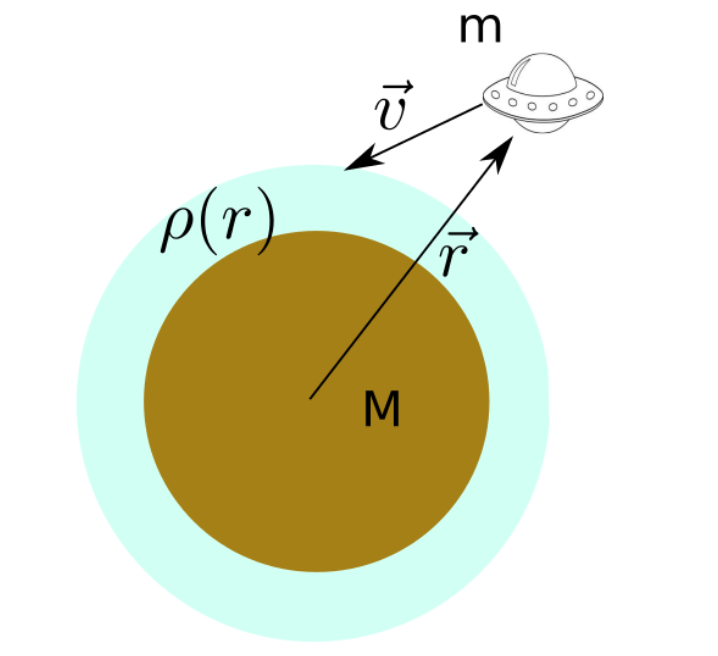
\includegraphics[scale=0.4]{media/landing.png}\\
\column{0.5\textwidth}
\small Velkommen til del 1B! Etter at du har skutt raketten din ut i rommet, så skal vi i denne delen beregne banen til både romfartøyet ditt og planeten som du skal besøke. Vi skal se på både analytiske og numeriske baneberegninger og prøve å forstå hva som avgjør banen til et objekt. Vi skal, kun ved å ta utgangspunkt i Newtons lover, utlede analytisk at planeter går i ellipsebaner, og se at det faktisk også finnes andre baner. Numerisk baneberegning har du kanskje gjort før med Eulers metode. Det blir litt repetisjon før vi tar det videre. \\{\bf Er du klar?}\\
\vspace*{0.5cm}
{\bf Dette forelesningsnotatet tilsvarer en og en halv fysisk dobbelttime, og kanskje litt mer}\\
\vspace*{1cm}\hyperlink{intro2}{\pagebutton{Neste side}}

%\movie[autostart]{testmovie}{launch.gif}%bate2.mpg
\end{columns}
\end{frame}

\begin{frame}
\label{intro2}
\begin{columns}
\column{0.5\textwidth}
%\hyperlink{intro}{\pagebutton{Forrige side}}\ \ \ \ \ \nextpage \\
\lastpagebutton{intro}
\addtocounter{pageno}{-1}
\vspace{0.5cm}
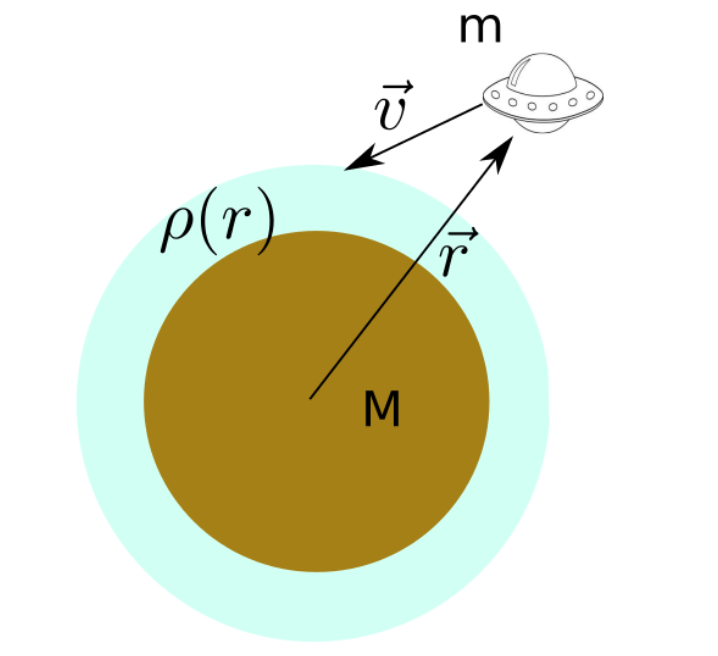
\includegraphics[scale=0.4]{media/landing.png}\\
Oppgave 1B8 som er en av innleveringsoppgavene går ut på å myklande en romsonde på en planet med atmosfære som illustert i figuren. I løpet av dette forelesningsnotatet vil du lære det du trenger for å løse denne oppgaven og mer til.
\column{0.5\textwidth}
Men før vi setter igang så skal vi varme opp litt med å fort sjekke at vi har kunnskapen fra del 1A på plass, samt se hva du allerede kan om temaene i del 1B.
\href{https://nettskjema.no/a/155530}{\begin{minipage}{5cm}Trykk her for å varme opp\end{minipage}}\\
Har du varmet opp? Er du svett og klar til å starte kampen? ...og sendt inn skjemaet?
\href{https://nettskjema.no/a/155530}{\choicebutton{Nei}}\ \ \ \ \hyperlink{intro2_b}{\choicebutton{Ja}}\\
\textcolor{white}{Neste side}
\end{columns}
\end{frame}

\begin{frame}
\label{intro2_b}
\begin{columns}
\column{0.5\textwidth}
%\hyperlink{intro}{\pagebutton{Forrige side}}\ \ \ \ \ \nextpage \\
\lastpagebutton{intro}
\addtocounter{pageno}{-1}
\vspace{0.5cm}
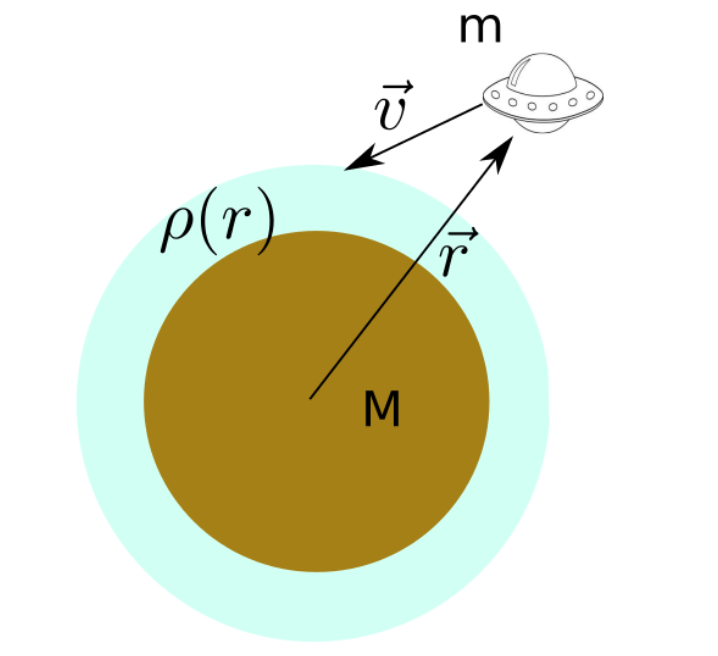
\includegraphics[scale=0.4]{media/landing.png}\\
Oppgave 1B8 som er en av innleveringsoppgavene går ut på å myklande en romsonde på en planet med atmosfære som illustert i figuren. I løpet av dette forelesningsnotatet vil du lære det du trenger for å løse denne oppgaven og mer til.
\column{0.5\textwidth}
Men før vi setter igang så skal vi varme opp litt med å fort sjekke at vi har kunnskapen fra del 1A på plass, samt se hva du allerede kan om temaene i del 1B.
\href{https://nettskjema.no/a/155530}{\begin{minipage}{5cm}Trykk her for å varme opp\end{minipage}}\\
Har du varmet opp? Er du svett og klar til å starte kampen? ...og sendt inn skjemaet?
\href{https://nettskjema.no/a/155530}{\choicebutton{Nei}}\ \ \ \ {\choicebutton{Ja}}\\
\hyperlink{blue_nytema1}{\pagebutton{Neste side}}
\end{columns}
\end{frame}


\renewcommand{\headline}{\small Numerisk løsning}
{
\setbeamercolor{background canvas}{bg=blue}
\begin{frame}
\label{blue_nytema1}
\hyperlink{intro}{\pagebutton{\small Forrige side}}
\nytemaside{euler4}
\textcolor{yellow}{Vi skal begynne med numeriske baneberegninger}\\
\vspace*{0.5cm}
\hyperlink{basicfysikk1a}{\pagebutton{Høres kjent ut, men la oss se da...}}
\end{frame}
}




\begin{frame}
\label{basicfysikk1a}
\dlastpagebutton{intro2}
La oss begynne med beina godt plantet på jorda. Og med litt {\bf veldig} grunnleggende videregåendeskole-fysikk (sorry!).
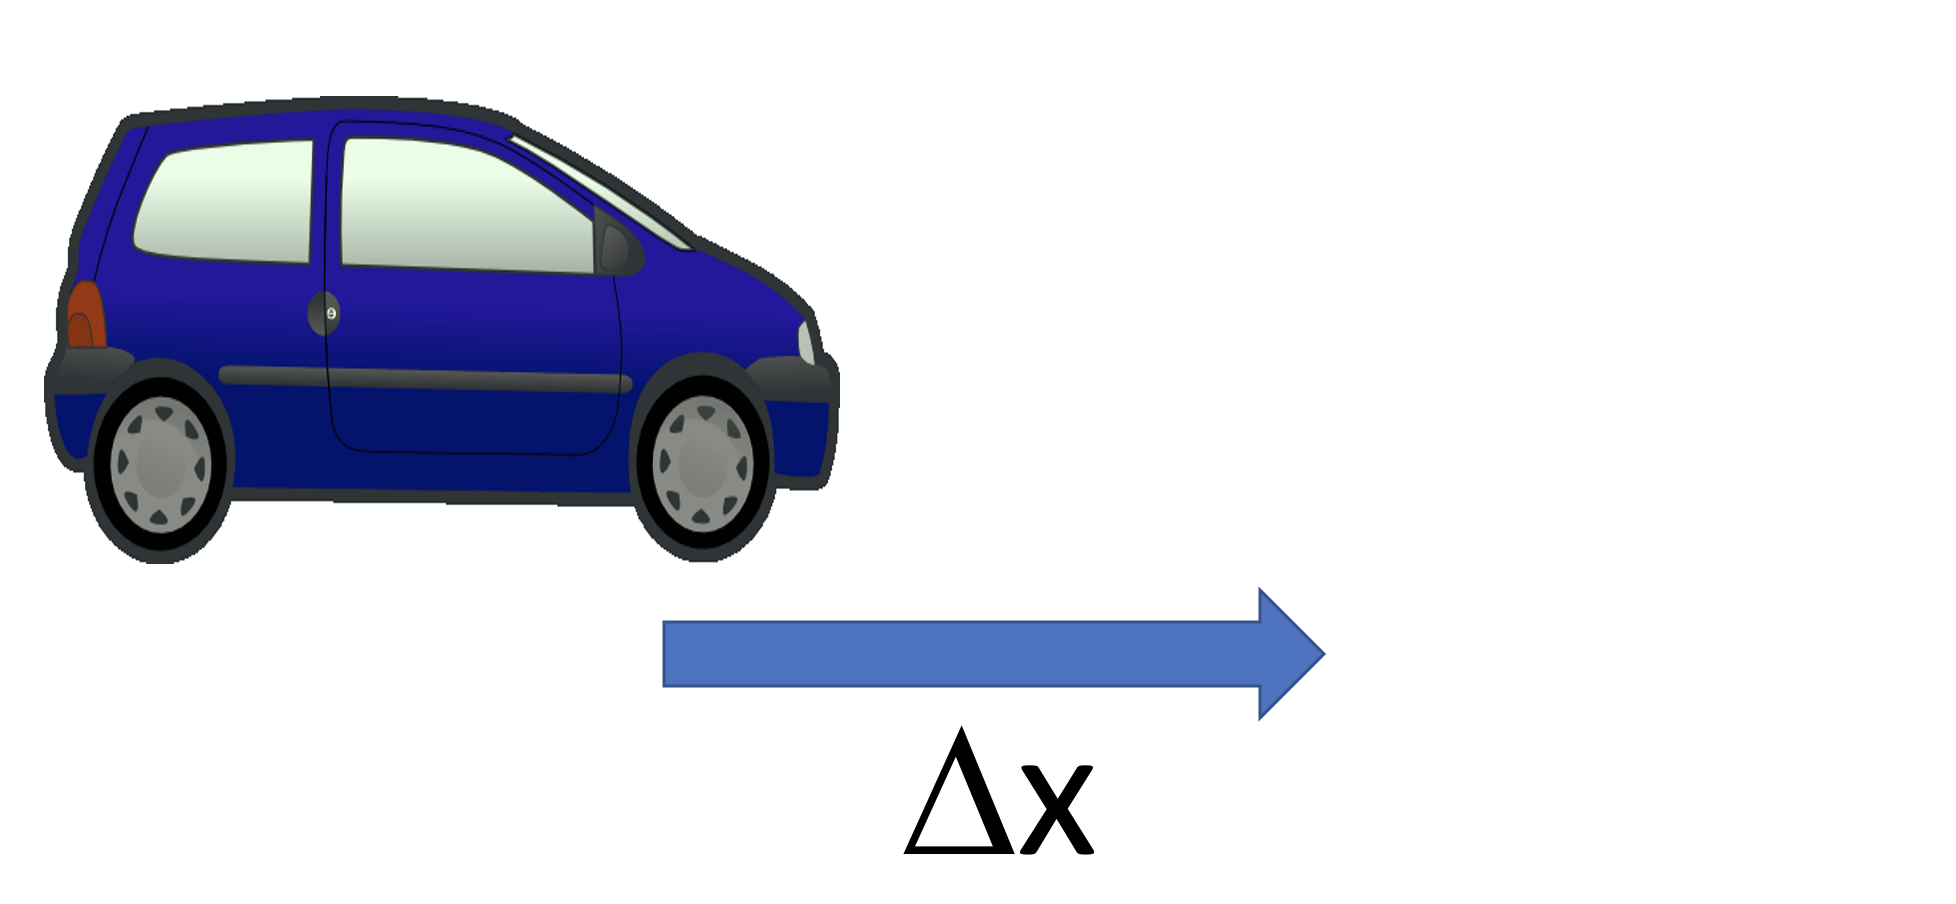
\includegraphics[scale=0.2]{media/car_move_1.png}\\
I figuren ser du en bil som beveger seg med konstant hastighet $v$. Hvilken avstand $\Delta x$ har denne bilen beveget seg i løpet av tiden $\Delta t$?\\
\hyperlink{basicfysikk1b}{\choicebutton{Trykk her når du har svaret!}}\\
\end{frame}


\begin{frame}
\label{basicfysikk1b}
\clastpagebutton{intro2}
La oss begynne med beina godt plantet på jorda. Og med litt {\bf veldig} grunnleggende videregåendeskole-fysikk (sorry!).
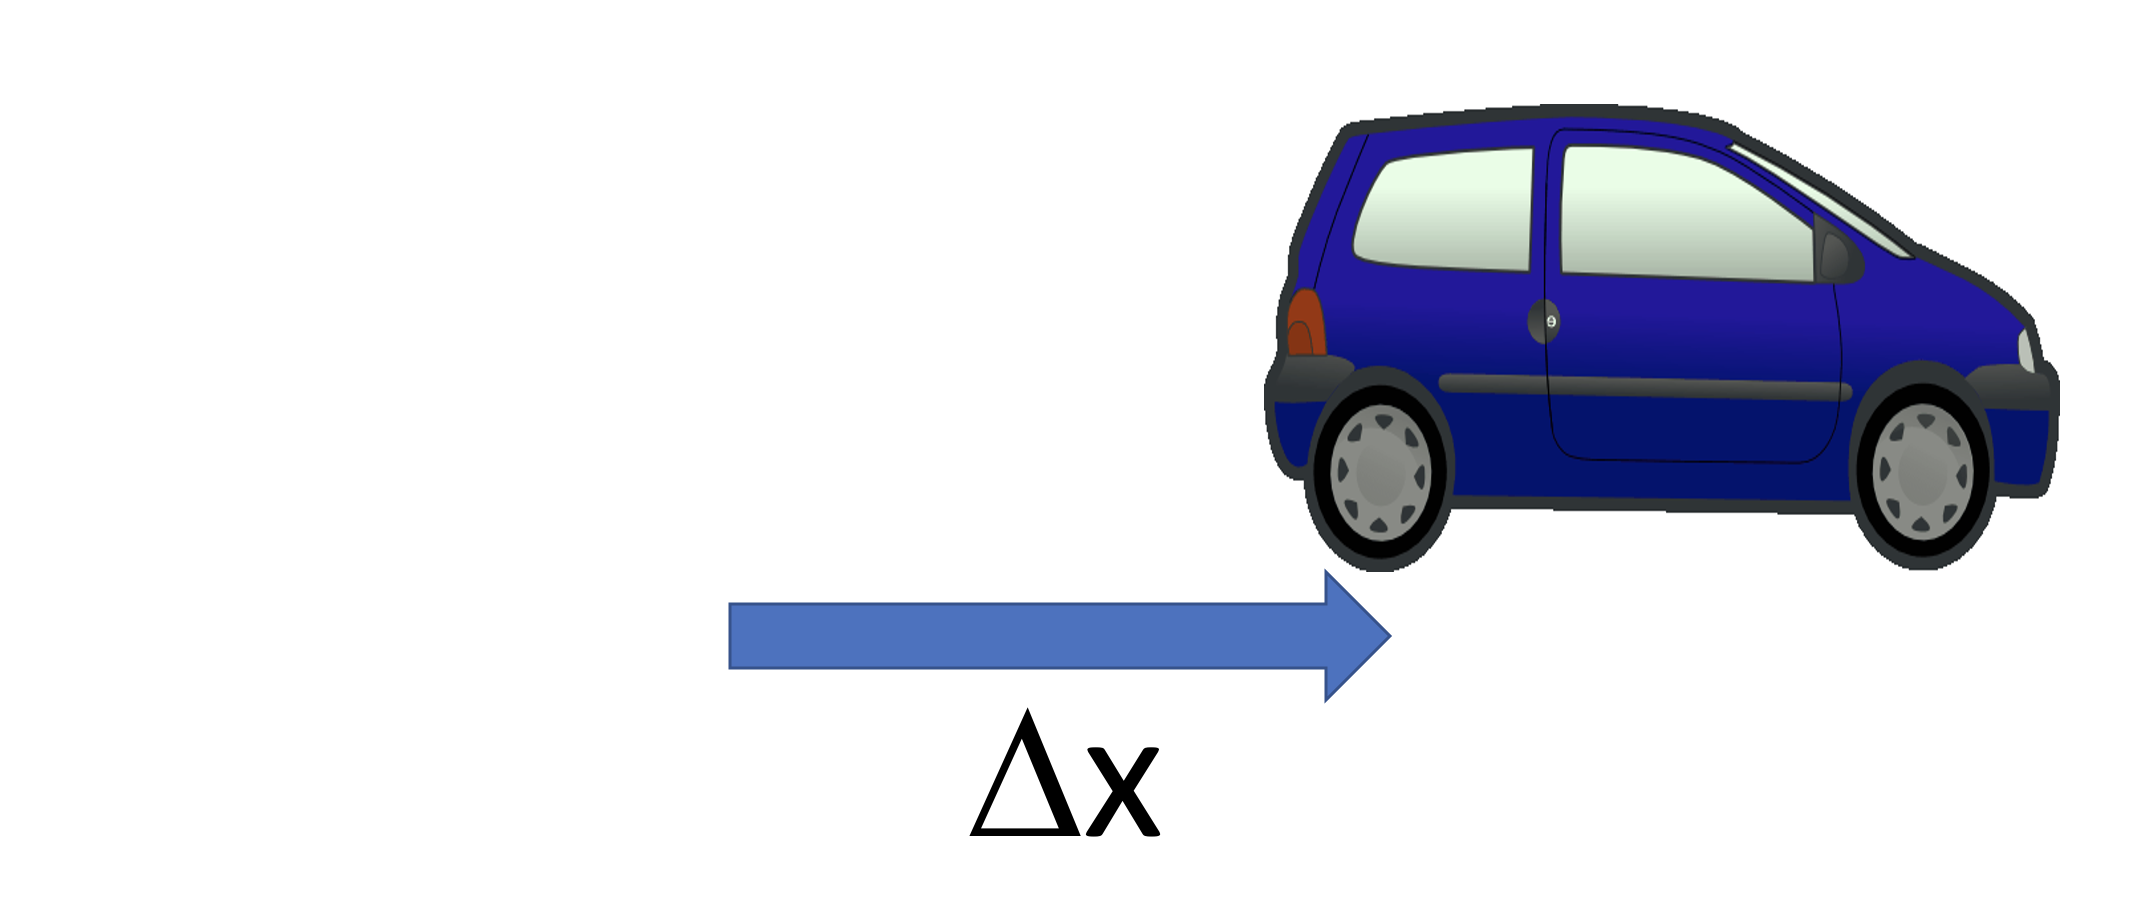
\includegraphics[scale=0.2]{media/car_move_2.png}\\
I figuren ser du en bil som beveger seg med konstant hastighet $v$. Hvilken avstand $\Delta x$ har denne bilen beveget seg i løpet av tiden $\Delta t$?\\
\textcolor{orange}{Ganske riktig ja, strekning er hastighet ganger tid, dermed er $\Delta x = v \Delta t$.}\\
\hyperlink{basicfysikk2a}{\pagebutton{Neste side}}
\end{frame}


\begin{frame}
\label{basicfysikk2a}
\begin{columns}
\column{0.5\textwidth}
\lastpagebutton{basicfysikk1a}
Nå har vi samme situasjon en gang til, men med vektorer. En romskip har posisjonsvektor $\vec{r}$. Vi skal i resten av dette emnet bruke konseptet {\it posisjonsvektor} ganske mye.
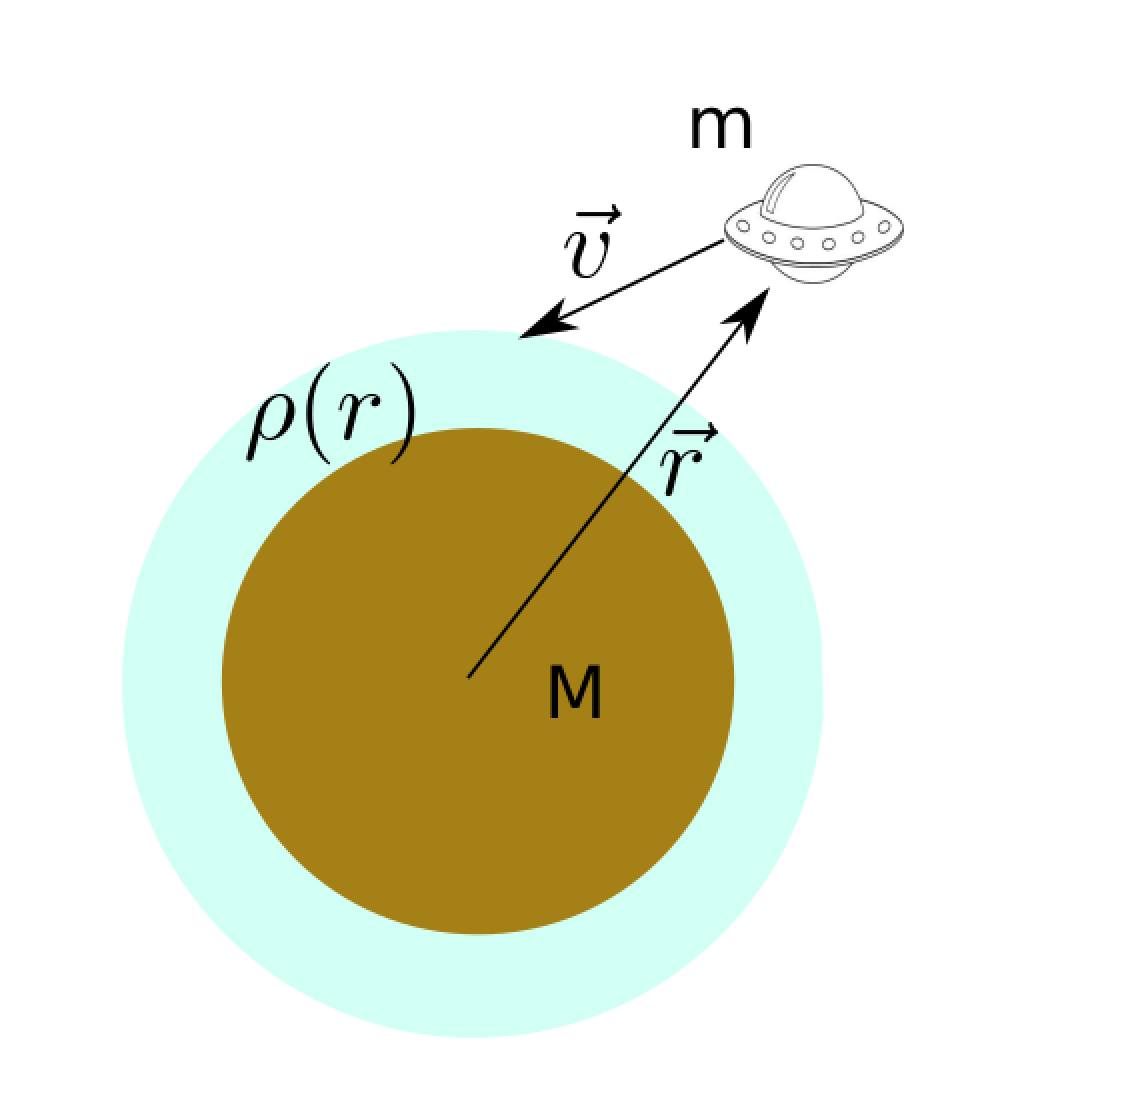
\includegraphics[scale=0.3]{media/spaceship_move_1.png}\\
\column{0.5\textwidth}
\vspace*{0.5cm}\\
\begin{alertblock}{\bf En posisjonsvektor...}
... er en vektor som peker fra origo i koordinatsystemet ditt til den posisjonen der objektet du studerer er. Når objektet endrer posisjon så endrer også posisjonsvektoren seg tilsvarende slik at den alltid peker på objektets posisjon.
\end{alertblock}
I figuren ser du dermed at vi har satt origo i sentrum av planeten. Romskipet har hastighetsvektor $\vec{v}$.  Hva er forflytningen $\Delta\vec{r}$ (altså endringsvektoren til posisjonsvektoren) som romskipet får i løpet av tid $\Delta t$?
\hyperlink{basicfysikk2b}{\choicebutton{Trykk her når du har svaret!}}\\
\end{columns}
\end{frame}

\begin{frame}
\label{basicfysikk2b}
\begin{columns}
\column{0.5\textwidth}
\clastpagebutton{basicfysikk1a}
Nå har vi samme situasjon en gang til, men med vektorer. En romskip har posisjonsvektor $\vec{r}$. Vi skal i resten av dette emnet bruke konseptet {\it posisjonsvektor} ganske mye.
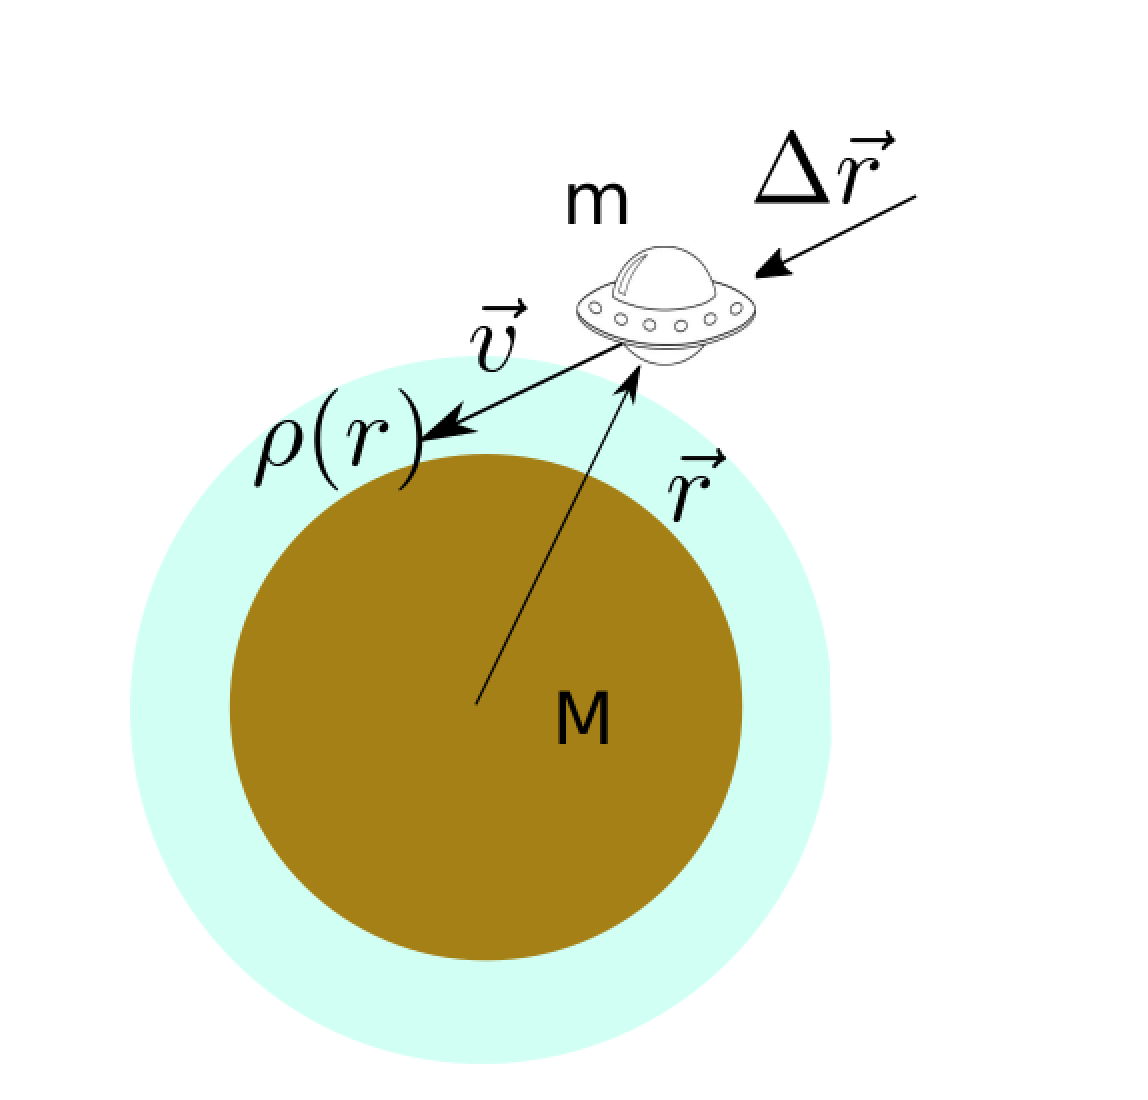
\includegraphics[scale=0.3]{media/spaceship_move_2.png}\\
\column{0.5\textwidth}
\vspace*{0.5cm}\\
\begin{alertblock}{\bf En posisjonsvektor...}
... er en vektor som peker fra origo i koordinatsystemet ditt til den posisjonen der objektet du studerer er. Når objektet endrer posisjon så endrer også posisjonsvektoren seg tilsvarende slik at den alltid peker på objektets posisjon.
\end{alertblock}
I figuren ser du dermed at vi har satt origo i sentrum av planeten. Romskipet har hastighetsvektor $\vec{v}$.   Hva er forflytningen $\Delta\vec{r}$ som romskipet får i løpet av tid $\Delta t$?
\textcolor{orange}{Ganske riktig ja, strekningsvektor er hastighetsvektor ganger tid, dermed er $\Delta\vec{r} = \vec{v} \Delta t$.}\\
\hyperlink{euler1}{\pagebutton{Neste side}}
\end{columns}
\end{frame}


\begin{frame}
\label{euler1}
\begin{columns}
\column{0.5\textwidth}
\lastpagebutton{basicfysikk2a}
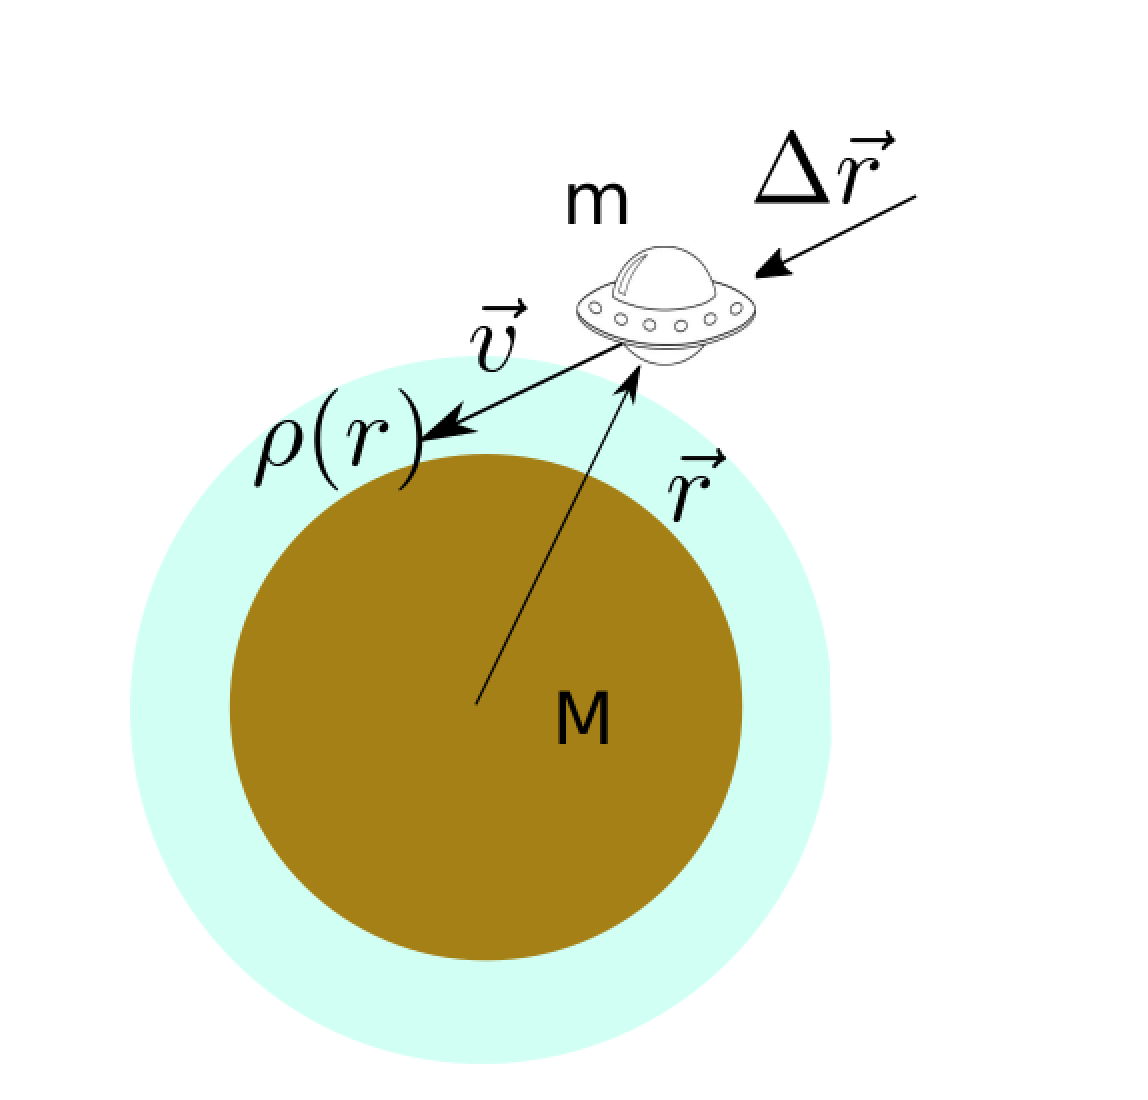
\includegraphics[scale=0.2]{media/spaceship_move_2.png}\\
Vi fant at forflytningen er $\Delta\vec{r}=\vec{v}\Delta t$. Hvis vi kaller opprinnelig posisjon for $\vec{r}_0$ og ny poisjon for $\vec{r}_1$, så har vi altså:
\[
\vec{r}_1  = \vec{r}_0 + \vec{v}\Delta t
\]
noe du sikkert kjenner som Eulers metode? Du har i tidligere emner brukt Eulers metode numerisk. 
\column{0.5\textwidth}
La oss se på hastighetsendring på samme måte:\\
Vi vet at akselerasjon er endring i hastighet per tid, slik at hvis du har en konstant akselerasjon $\vec{a}$, så vil endring i hastighet i løpet av tid $\Delta t$ per definisjon være gitt ved
\[
\Delta\vec{v} = \vec{a}\Delta t
\]
Hvis opprinnelig hastighet var $\vec{v}_0$ og ny hastighet er $\vec{v}_1$ så har vi
\[
\vec{v}_1  = \vec{v}_0 + \vec{a}\Delta t
\]
... og dermed har vi Eulers metode for å oppdatere hastigheten også!
\hyperlink{euler2}{\pagebutton{Neste side}}
\end{columns}
\end{frame}

\begin{frame}
\label{euler2}
\lastpagebutton{euler1}
Dette var repetisjon, men kanskje en mer fysisk måte å utlede det på enn du er vant til? Det er viktig å forstå de fysiske prinsippene bak når vi nå etterhvert skal ta dette videre. 
\begin{block}{\bf Numerisk beregning av forflytning og hastighetsendring...}
Når du gjør dette numerisk, husk også at det er mer nøyaktig å bruke Euler-Cromers metode, dvs. at du oppdaterer posisjonen med den nye hastigheten, dvs.
\begin{align}
\vec{v}_1  &= \vec{v}_0 + \vec{a}\Delta t\\
\vec{r}_1  &= \vec{r}_0 + \vec{v_1}\Delta t
\end{align}
\end{block}
\hyperlink{euler3}{\pagebutton{Neste side}}
\end{frame}

\begin{frame}
\label{euler3}
\lastpagebutton{euler2}
Merk at det du har gjort her matematisk er jo å løse likningssystemene 
\[
\frac{d\vec{r}}{dt}=\vec{v}\ \ \ \ \ \frac{d\vec{v}}{dt}=\vec{a}
\]
{\bf (disse likningssystemene er jo bare definisjonene av hastighet og akselrasjon, ser du det?)}
Du kommer frem til samme resultat hvis vi gjør de infinitsimale størrelsene endelige (men fortsatt små) ved å kalle $dt$ for $\Delta t$, etc:
\[
\frac{\Delta\vec{r}}{\Delta t}=\vec{v}\ \ \ \ \ \frac{\Delta\vec{v}}{\Delta t}=\vec{a}
\]
Hvis du ganger opp med $\Delta t$ på begge sider av likningene her, så ender du igjen opp med det samme som på de forrige slidene. Merk deg denne måten å tenkte på da du vil bruke den til å løse andre typer differensiallilkninger senere.\\
{\bf Da er repetisjonen over, nå begynner moroa her...}\\
\hyperlink{blue_nytema2}{\pagebutton{Neste side}}
\end{frame}

\renewcommand{\headline}{\small Forberede 2-legemeproblem: enhetsvektorer}
{
\setbeamercolor{background canvas}{bg=blue}
\begin{frame}
\label{blue_nytema2}
\hyperlink{euler3}{\pagebutton{\small Forrige side}}
\nytemaside{hastighet1}
\textcolor{yellow}{\tiny Nå skal vi begynne med en laaaaang analytisk utledning her som til slutt ender opp med bevis for at planeter går i ellipsebaner. Vi går gjennom utledningen fordi (1) det er virkelig morsomt og faktisk ha utledet dette fra scratch, hører med til allmenndannelsen og (2) fordi mange av tingene vi bruker underveis i utledningen er viktige metoder i matematikk og fysikk som vi skal bruke mange ganger i AST2000 og også ting som skal brukes i numeriske beregninger for å få de til å gå fortere. Vi begynner med å definere et nytt sett med enhetsvektorer i planet. }\\
\vspace*{0.5cm}
\hyperlink{euler4}{\pagebutton{Ok, jeg er klar!}}
\end{frame}
}

\begin{frame}
\label{euler4}
\lastpagebutton{euler3}
Det vi har gjort så langt er å se hvordan vi kan finne romskipets bevegelse numerisk, steg for steg. Nå skal vi se på hvordan dette kan gjøres analytisk. Det er viktig å gjøre ting analytisk der det kan gjøres analytisk fordi du da kan gjøre ting mye raskere på datamaskin og samtidig få en mye dypere innsikt i fysikken bak. Og ikke minst, det er jo litt kult å faktisk ha utledet at planeter har ellipsebaner helt fra scratch?\\
\vspace*{0.5cm}
Utledningen av løsningen på dette {\bf 2-legemeproblemet} (og det er kun for 2 legemer at vi kan løse dette analytisk) er en ganske omfattende utledning, men på veien dit kommer vi innom mange temaer som vi skal bruke igjen og igjen i løpet av kurset, så det er viktig å forstå detaljene her.\\
Trenger du en pause, så ta den nå! Trekk pusten godt!\\
{\bf Er du klar?}
\hyperlink{riktig_klar}{\choicebutton{{\bf Ja, kom igjen!}}}\ \ \ \ \hyperlink{red_pyse}{\choicebutton{Tjjjaaaaa....}}\
\end{frame}

{
\setbeamercolor{background canvas}{bg=red}
\begin{frame}
\label{red_pyse}
\lastpagebutton{euler4}
\vspace*{2cm}
\textcolor{white}{\Huge PYSE!}\\
\end{frame}
}

{
\setbeamercolor{background canvas}{bg=yellow}
\begin{frame}
\label{riktig_klar}
\clastpagebutton{euler4}
\vspace*{2cm}
Se det, det var riktig instilling ja!
Moroa begynner på ...
\hyperlink{enhetsvektorer1}{\pagebutton{.. neste side}}
\end{frame}
}


\begin{frame}
\label{enhetsvektorer1}
\begin{columns}
\column{0.5\textwidth}
\lastpagebuttonx{euler4}
\hspace*{-0.5cm}\headlinebutton{\headline}\\
Før vi begynner på selve utledningen så må vi innom et par småting som forberedelse til utledningen, la oss begynne med koordinatsystemer og enhetsvektorer.\\
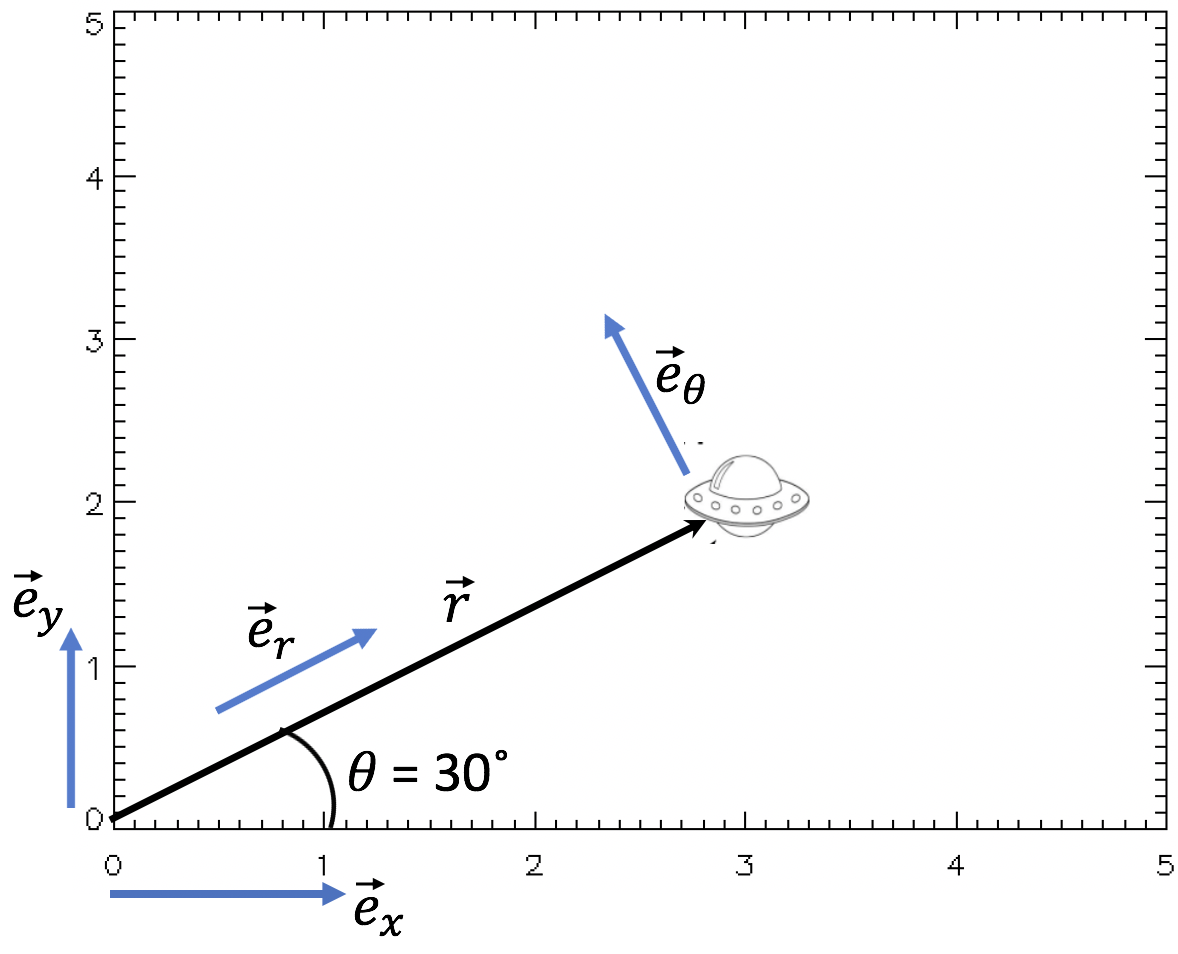
\includegraphics[scale=0.3]{media/unity_vectors.png}\\
\column{0.5\textwidth}
Her ser du posisjonsvektoren $\vec{r}$ til romskipet samt enhetsvektorene $\vec{e}_x$ og $\vec{e}_y$. Dette er de samme enhetsvektorene som du kaller for $\vec{i}$ og $\vec{j}$ i andre fag. (vi bruker andre navn på dem her for å skape litt forvirring)\\

Se for øyeblikket bort ifra andre ting på figuren. Vi starter med litt oppvarming igjen. Vi skal skrive posisjonsvektoren $\vec{r}$ ved hjelp av enhetsvektorene
\[
\vec{r} = a\vec{e}_x + b\vec{e}_y
\]
Hva er $a$ og $b$ her?\\
\hyperlink{feilxy}{\choicebutton{{$a=1\ b=1$}}}\ \ \hyperlink{riktigxy}{\choicebutton{$a=3\ b=2$}}\ \ \hyperlink{feilxy}{\choicebutton{$a=2\ b=3$}}\ \ \hyperlink{feilxy}{\choicebutton{$a=0\ b=0$}}
\end{columns}
\end{frame}

{
\setbeamercolor{background canvas}{bg=black}
\begin{frame}
\label{feilxy}
\lastpagebutton{enhetsvektorer1}
\textcolor{white}{Det ble galt! Er du sikker på at du forstår hva det spørres om? Innser du at $a$ og $b$ her er x- og y-komponentene til vektoren $\vec{r}$? Det er helt essensielt at du forstår dette før du går videre. Spør gruppelærer eller foreleser hvis du har den minste tvil. Gå tilbake og forsikre deg om at du forstår før du går videre!}
\end{frame}
}

{
\setbeamercolor{background canvas}{bg=yellow}
\begin{frame}
\label{riktigxy}
\begin{columns}
\column{0.5\textwidth}
\clastpagebutton{enhetsvektorer1}
{\bf STEMMER!}.Vi ser på figuren igjen:
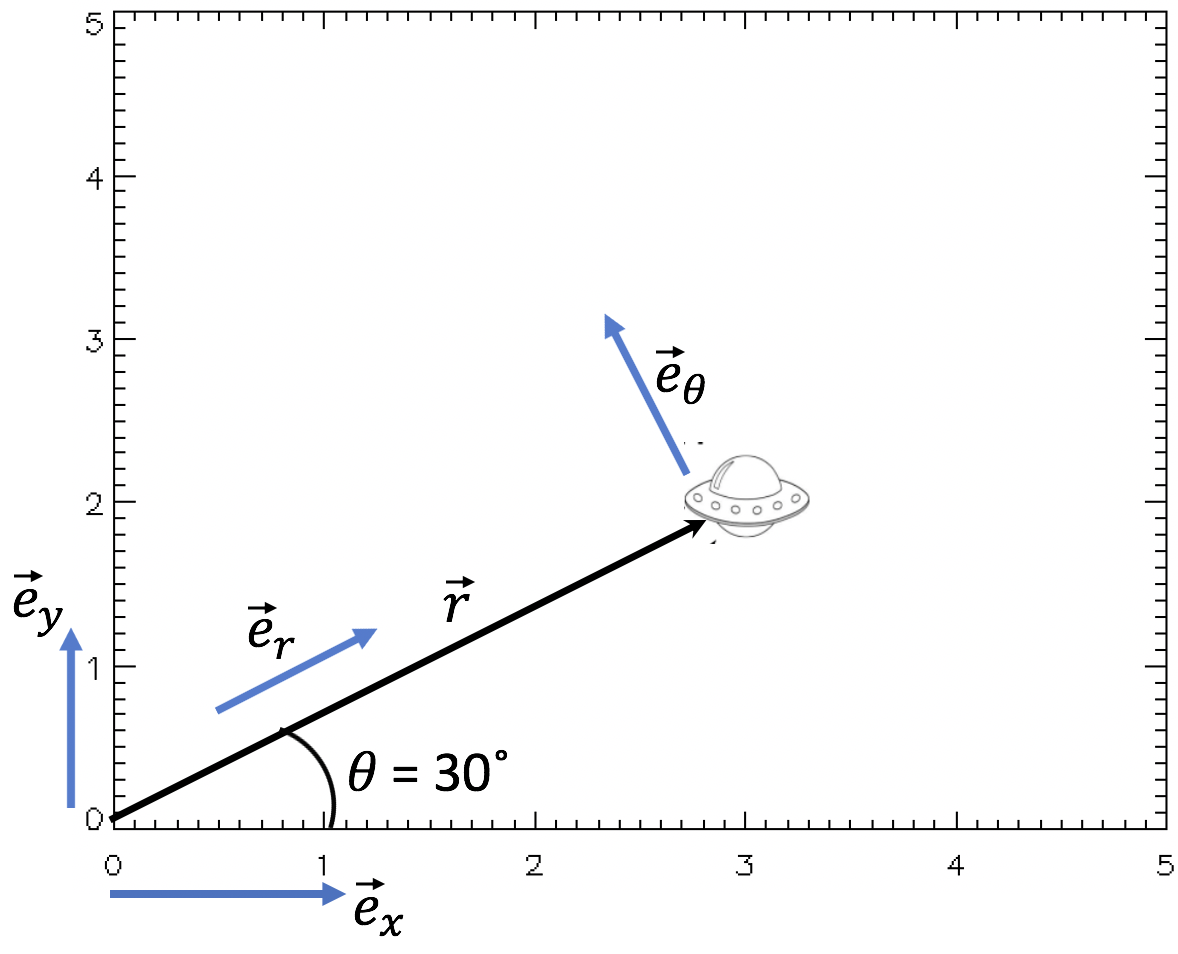
\includegraphics[scale=0.26]{media/unity_vectors.png}\\

Ser du at det er tegnet inn to andre enhetsvektorer $\vec{e}_r$ og $\vec{e}_\theta$? Dette er enhetsvektorer som fortsatt har lengde 1, men som peker {\bf langs} $\vec{r}$ og {\bf ortogonalt} med $\vec{r}$. 

{\small Merk at hvis f.eks. romskipet har en positiv hastighetskomponent langs $\vec{e}_\theta$ så vil vinkelen $\theta$ øke med tiden.}\\
\column{0.5\textwidth}
\\`
Vi kan altså representere vektoren $\vec{r}$ med enten x-y enhetsvektorer eller r-$\theta$ enhetsvektorer (nå ser du kanskje at det nye navnet på $\vec{i}$ og $\vec{j}$ faktisk {\bf ikke} var for å forvirre deg, men har en mening!)\\
Du kan dermed representere en vektor enten med komponentene langs x-y enhetsvektorene eller med komponentene langs r-$\theta$ enhetsvektorene. Ved første øyesyn kan det kanskje virke som at det er likegyldig hvilket av systemene du velger, men det er en stor grunnleggende forskjell mellom disse to koordinatsystemene. Hvilken?
\textcolor{red}{Tenk deg godt om før du går til neste side der svaret står!}
\hyperlink{enhetsvektorer2}{\pagebutton{Neste side}}
\end{columns}
\end{frame}
}


\begin{frame}
\label{enhetsvektorer2}
\lastpagebutton{riktigxy}
\addtocounter{pageno}{-1}
Et lite hint før du får svaret: Hva skjer med enhetsvektorene dersom romskipet beveger seg? Er det en grunnleggende forskjell mellom x-y-enhetsvektorene og r-$\theta$-enhetsvektorene da? \textcolor{red}{Tenk deg om og ...} \hyperlink{enhetsvektorer2_b}{\choicebutton{trykk her}}\\
\textcolor{white}{Ganske riktig! r-$\theta$-enhetsvektorene endrer seg med tiden når objektet de peker på endrer posisjon! De er tidsavhengige enhetsvektorer, mens x-y-enhetsvektorene ikke endrer seg.
Men dette gjør det vel mer komplisert å bruke r-$\theta$-enhetsvektorene? Hva iallverden skal vi med disse da? Kan du tenkte deg noen fordeler med dem?}\\
\textcolor{white}{Tenk deg godt om før du går til ... }\\
\textcolor{white}{... neste side}
\end{frame}


\begin{frame}
\label{enhetsvektorer2_b}
\lastpagebutton{riktigxy}
\addtocounter{pageno}{-1}
Et lite hint før du får svaret: Hva skjer med enhetsvektorene dersom romskipet beveger seg? Er det en grunnleggende forskjell mellom x-y-enhetsvektorene og r-$\theta$-enhetsvektorene da? \textcolor{red}{Tenk deg om og ...} {\choicebutton{trykk her}}\\
Ganske riktig! r-$\theta$-enhetsvektorene endrer seg med tiden når objektet de peker på endrer posisjon! De er tidsavhengige enhetsvektorer, mens x-y-enhetsvektorene ikke endrer seg.
Men dette gjør det vel mer komplisert å bruke r-$\theta$-enhetsvektorene? Hva iallverden skal vi med disse da? Kan du tenkte deg noen fordeler med dem?\\
\textcolor{red}{Tenk deg godt om før du går til ... }
\hyperlink{enhetsvektorer3}{\pagebutton{... neste side}}
\end{frame}

\begin{frame}
\label{enhetsvektorer3}
\lastpagebutton{enhetsvektorer2}
Vi skal se på fordelene etterhvert, men la oss prøve å bruke dem:
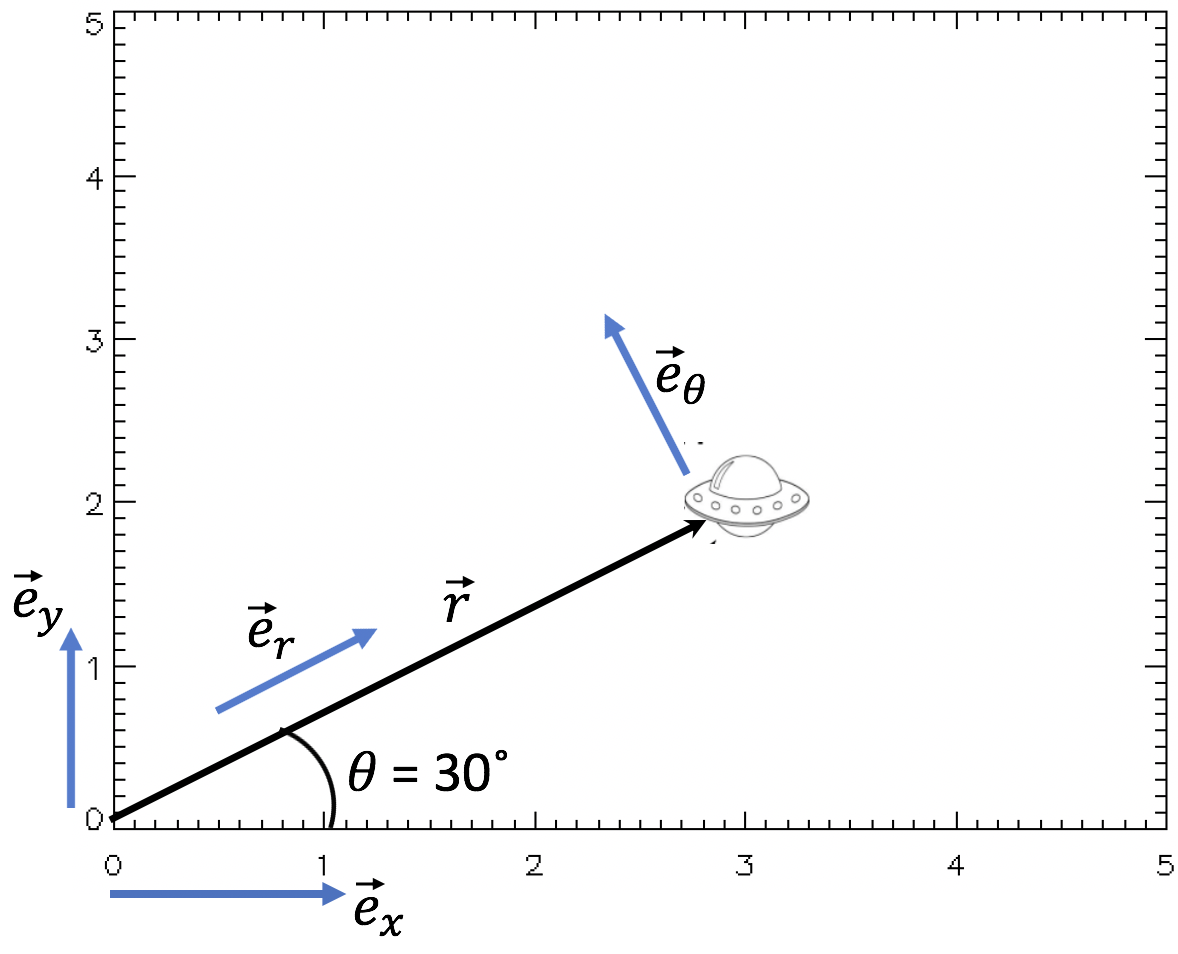
\includegraphics[scale=0.28]{media/unity_vectors.png}\\
Hvis vi nå skal skrive poisjonsvektoren $\vec{r}$ uttrykt ved de nye enhetsvektorne:
\[
\vec{r} = a\vec{e}_r+b\vec{e}_\theta
\]
hva blir da $a$ og $b$?
\hyperlink{feilrt}{\choicebutton{{$a=1\ b=1$}}}\ \ \hyperlink{feilrt}{\choicebutton{$a=3\ b=2$}}\ \ \hyperlink{feilrt}{\choicebutton{$a=\sqrt{13}\ b=\sqrt{13}$}}\ \ \hyperlink{riktigrt}{\choicebutton{$a=\sqrt{13}\ b=0$}}\ \ \hyperlink{feilrt}{\choicebutton{$a=0\ b=\sqrt{13}$}}\ \ \hyperlink{feilrt}{\choicebutton{$a=\sqrt{13}\ b=30$}}\ \ \hyperlink{feilrt}{\choicebutton{$a=\sqrt{13}\ b=1$}}
\end{frame}


{
\setbeamercolor{background canvas}{bg=black}
\begin{frame}
\label{feilrt}
\lastpagebutton{enhetsvektorer3}
\textcolor{white}{Det ble galt! Husk at r-$\theta$-koordinatsystemet funker helt på samme måte som x-y, altså du dekomponerer vektoren i de to enhetsvektorene. Dvs.
\begin{align}
a &= \vec{r}\cdot\vec{e}_r\\
b &= \vec{r}\cdot\vec{e}_\theta
\end{align}
Hjelper det deg? Prøv igjen med dette som utgangspunkt!
}
\end{frame}
}

{
\setbeamercolor{background canvas}{bg=yellow}
\begin{frame}
\label{riktigrt}
\clastpagebutton{enhetsvektorer3}
{\bf STEMMER!}.Vi ser på figuren igjen:\\
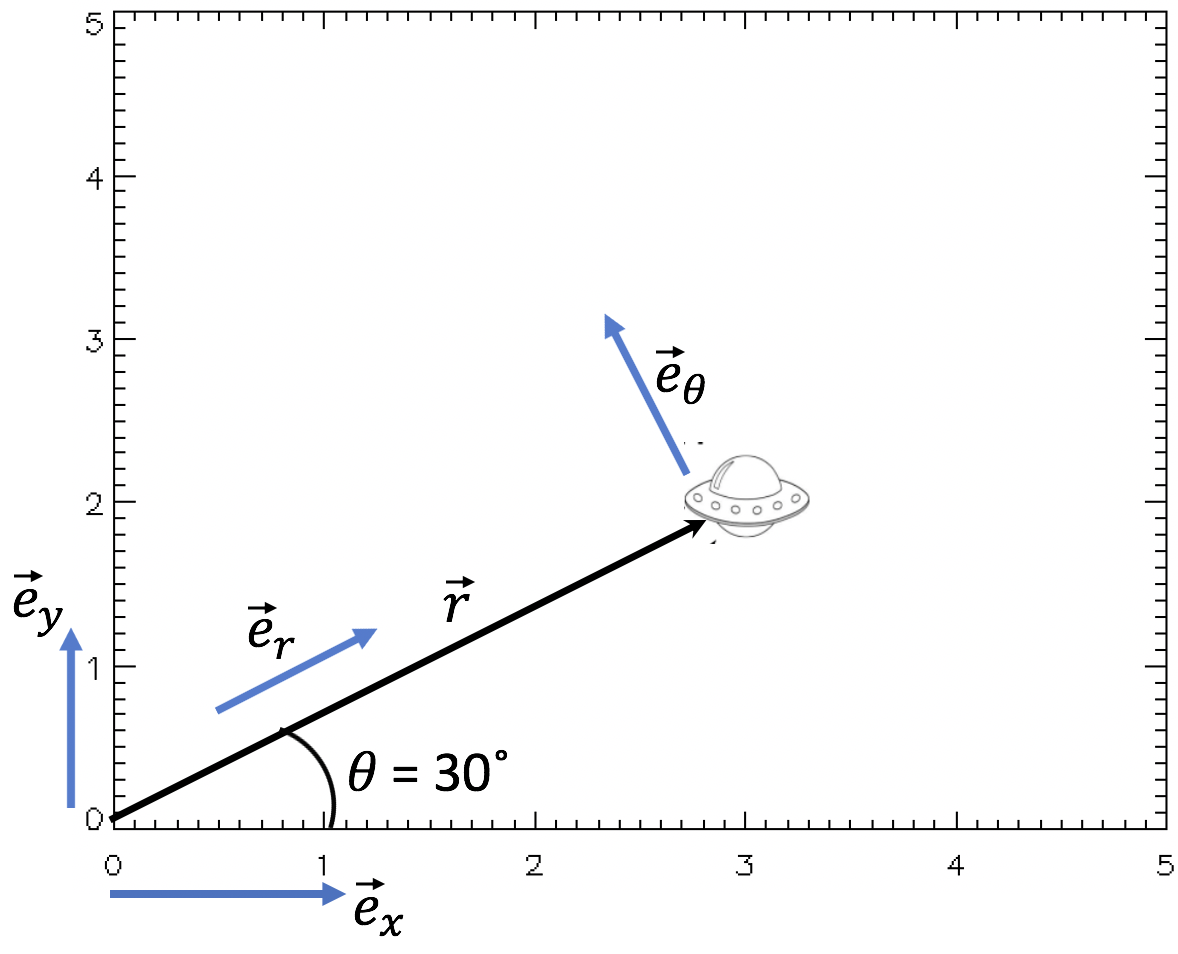
\includegraphics[scale=0.26]{media/unity_vectors.png}\\
Poisjonsvektoren har altså kun en komponent som går langs $\vec{e}_r$, ingen som går ortogonalt. Hvis vi tenker litt på det så er det egentlig opplagt siden $\vec{e}_r$ er definert fra $\vec{r}$.

\hyperlink{blue_nytema3}{\pagebutton{Neste side}}
\end{frame}
}

\renewcommand{\headline}{\small Forberede 2-legemeproblem: vektorregning}
{
\setbeamercolor{background canvas}{bg=blue}
\begin{frame}
\label{blue_nytema3}
\hyperlink{riktigrt}{\pagebutton{\small Forrige side}}
\nytemaside{hastighet4}
\textcolor{yellow}{Vi skal leke oss litt med våre nye enhetsvektorer. Og derivere vektorfunksjoner.}\\
\vspace*{0.5cm}
\hyperlink{hastighet1}{\pagebutton{Kuuult, sett igang!}}
\end{frame}
}

\begin{frame}
\label{hastighet1}
\lastpagebutton{blue_nytema3}
Det vi fant er altså at posisjonsvektoren kan skrives som 
\[
\vec{r}=r\vec{e}_r
\]
der $r=|\vec{r}|$. Enig?\\
Hvis du tar utgangspunkt i dette, hvordan vil du nå gå frem for å finne hastighetsvektoren $\vec{v}$ til romskipet, gitt at du kjenner $r(t)$ og $\theta(t)$?\\
{\bf MERK:} Det er ikke meningen at du skal regne ut hastighetsvektoren riktig enda, kun tenke gjennom hvordan du vil gå frem for å gjøre det!\\
Har du tenkt nøye gjennom hvordan du kunne tenke deg å gjøre det? Har du en ide? {\bf (tenk i maks 2-3 minutter)}\\
\hyperlink{riktig_nohintv}{\choicebutton{{Ja, jeg tror det!}}}\\
\hyperlink{red_hintv}{\choicebutton{tjaaaaa, et bittelite hint kanskje?}}
\end{frame}


{
\setbeamercolor{background canvas}{bg=red}
\begin{frame}
\label{red_hintv}
\lastpagebutton{hastighet1}
Hint skal bli:\\
Hva er definisjonen av hastighet? Den med en derivert?
\end{frame}
}

{
\setbeamercolor{background canvas}{bg=yellow}
\begin{frame}
\label{riktig_nohintv}
\lastpagebutton{hastighet1}
\addtocounter{pageno}{-1}
Var det noe alla:
\[
\vec{v}=\frac{d\vec{r}}{dt}
\]
du tenkte på?\\
 Hvordan går du videre her? (vi lærte vel akkurat hvordan uttrykke $\vec{r}$ med enhetsvektorer...)\\
 \hyperlink{riktig_nohintv_b}{\choicebutton{Har du en ide?}}\\
 \textcolor{yellow}{
Jepp, kjerneregel selvfølgelig. Da blir det vel:
\[
\vec{v}=\frac{d}{dt}(r\vec{e}_r)=\dot r\vec{e}_r+r\frac{d}{dt}\vec{e}_r
\]}
\textcolor{yellow}{\bf
Merk at vi skriver tidsderivert som en prikk over, dvs
\[
\dot r = \frac{dr}{dt}
\]
Dette skal vi bruke mye i resten av kurset, så lær deg dette med en gang!
}
\textcolor{yellow}{Neste side}
\end{frame}
}

{
\setbeamercolor{background canvas}{bg=yellow}
\begin{frame}
\label{riktig_nohintv_b}
\lastpagebutton{hastighet1}
Var det noe alla:
\[
\vec{v}=\frac{d\vec{r}}{dt}
\]
du tenkte på?\\
 Hvordan går du videre her? (vi lærte vel akkurat hvordan uttrykke $\vec{r}$ med enhetsvektorer...)\\
{\choicebutton{Har du en ide?}}\\
Jepp, kjerneregel selvfølgelig. Da blir det vel:
\[
\vec{v}=\frac{d}{dt}(r\vec{e}_r)=\dot r\vec{e}_r+r\frac{d}{dt}\vec{e}_r
\]
\textcolor{red}{\bf
Merk at vi skriver tidsderivert som en prikk over, dvs
\[
\dot r = \frac{dr}{dt}
\]
Dette skal vi bruke mye i resten av kurset, så lær deg dette med en gang!
}

\hyperlink{hastighet2}{\pagebutton{Neste side}}
\end{frame}
}


\begin{frame}
\label{hastighet2}
\lastpagebutton{riktig_nohintv}
Vi har altså:
\[
\vec{v}=\frac{d}{dt}(r\vec{e}_r)=\dot r\vec{e}_r+r\frac{d}{dt}\vec{e}_r
\]
Der vi trenger å finne {\it den tidsderiverte av enhetsvektoren!}. Dette er litt uvant, vanligvis er enhetsvektorer faste størrelser.
\begin{block}{Grublis}
Hvordan kan du går frem for å finne den tidsderiverte av enhetsvektoren $\vec{e}_r$??? Du kan uttrykke svaret med de tidsderiverte, $\dot r$ og $\dot\theta$ samt enhetsvektorer.
\end{block}
\hyperlink{hastighet3}{\pagebutton{Jeg har grublet maks 2 min. og er klar til å gå videre}}
\end{frame}

\begin{frame}
\label{hastighet3}
\lastpagebutton{hastighet2}
\addtocounter{pageno}{-1}
Første steg kan være å uttrykke $\vec{e}_r$ med faste enhetsvektorer som $\vec{e}_x$ og $\vec{e}_y$. La oss bruke denne figuren:
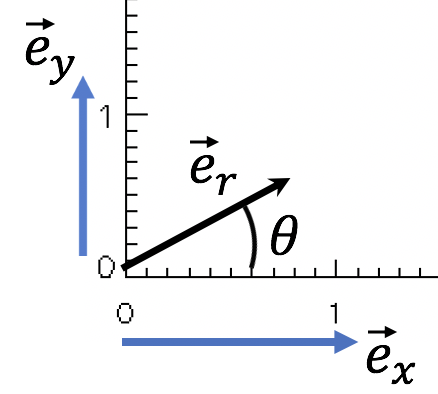
\includegraphics[scale=0.5]{media/unity_vector_decomp.png}\\
Hvis vi nå skal skrive
\[
\vec{e}_r=a\vec{e}_x+b\vec{e}_y
\]
Hva er $a$ og $b$?
Tenk deg litt om, før du ...
\hyperlink{hastighet3_b}{\choicebutton{... trykker her for noen alternativer}}\\
\textcolor{white}{
Er det:\\
{$a=\theta\  b = 0$}\ \ \ \ {$a=\sin{\theta}\  b = 0$}\ \ \ \ {$a=\cos{\theta}\ b=0$}\ \ \ \ {$a=\sin{\theta}\  b = \cos{\theta}$}\ \ \ \ \ {$a=\cos{\theta}\ b=\sin{\theta}$}\ \ \ \ {$a=1\ b=\sin{\theta}$}}
\end{frame}

\begin{frame}
\label{hastighet3_b}
\lastpagebutton{hastighet2}
\addtocounter{pageno}{-1}
Første steg kan være å uttrykke $\vec{e}_r$ med faste enhetsvektorer som $\vec{e}_x$ og $\vec{e}_y$. La oss bruke denne figuren:
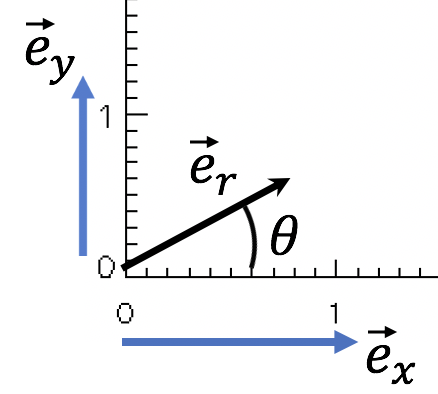
\includegraphics[scale=0.5]{media/unity_vector_decomp.png}\\
Hvis vi nå skal skrive
\[
\vec{e}_r=a\vec{e}_x+b\vec{e}_y
\]
Hva er $a$ og $b$?
Tenk deg litt om, før du ...
{\choicebutton{... trykker her for noen alternativer}}\\
Er det:\\
\hyperlink{feilerfeil}{\choicebutton{$a=\theta\  b = 0$}}\ \ \ \ \hyperlink{feilerfeil}{\choicebutton{$a=\sin{\theta}\  b = 0$}}\ \ \ \ \hyperlink{feilerfeil}{\choicebutton{$a=\cos{\theta}\ b=0$}}\ \ \ \ \hyperlink{feilerfeil}{\choicebutton{$a=\sin{\theta}\  b = \cos{\theta}$}}\ \ \ \ \hyperlink{riktigerrett}{\choicebutton{$a=\cos{\theta}\ b=\sin{\theta}$}}\ \ \ \ \hyperlink{feilerfeil}{\choicebutton{$a=1\ b=\sin{\theta}$}}
\end{frame}


{
\setbeamercolor{background canvas}{bg=black}
\begin{frame}
\label{feilerfeil}
\dlastpagebutton{hastighet3_b}
\textcolor{white}{Det ble galt! Husk at alt du gjør er å dekomponere $\vec{e}_r$ ned på x- og y-aksene. Husk også at lengden av $\vec{e}_r$ er 1. Hvis du har en hvilken som helst vektor med kjent lengde og du skal finne x- og y-komponentene, hva gjør du vanligvis?\\
Prøv å ha dette i tankene når du nå går tilbake og gjør et nytt forsøk.\\
Hvis du ikke forstår dette, ta kontakt med gruppelærer eller foreleser!}
\end{frame}
}

{
\setbeamercolor{background canvas}{bg=yellow}
\begin{frame}
\label{riktigerrett}
\clastpagebutton{hastighet3}
{\bf STEMMER!}. Når vi dekomponerer $\vec{e}_r$ ned på x- og y-aksen så er x- og y-komponentene av en vektor med lengde 1 lik cosinus og sinus til vinkelen, akkurat slik vi er vant til, dermed
\[
\vec{e}_r = \cos{\theta}\vec{e}_x+\sin{\theta}\vec{e}_y
\]
Man kan vise helt tilsvarende at
\[
\vec{e}_\theta = -\sin{\theta}\vec{e}_x+\cos{\theta}\vec{e}_y
\]
(hvordan kan du sjekke om disse er ortogonale?)\\
Nå har du fått god hjelp til å derivere $\vec{e}_r$ med hensyn på tiden. Gjør regningen på papir (eller i hodet) og se om du finner et av følgende svar:\\
\hyperlink{feilderfeil}{\choicebutton{$\dot{\vec{e}}_r = \vec{e}_\theta$}}\ \ \ \ \hyperlink{feilderfeil}{\choicebutton{$\dot{\vec{e}}_r=\cos{\theta}\vec{e}_r$}}\ \ \ \ \hyperlink{feilderfeil}{\choicebutton{$\dot{\vec{e}}_r=-\sin{\theta}\vec{e}_\theta$}}\ \ \ \ \hyperlink{riktigderrett}{\choicebutton{$\dot{\vec{e}}_r=\dot\theta\vec{e}_\theta$}}\ \ \ \ \hyperlink{feilderfeil}{\choicebutton{$\dot{\vec{e}}_r=\dot\theta\vec{e}_r+\theta\vec{e}_r$}}\ \ \ \ \hyperlink{feilderfeil}{\choicebutton{$\dot{\vec{e}}_r=\dot\theta\sin{\theta}\vec{e}_r$}}
\end{frame}
}


{
\setbeamercolor{background canvas}{bg=black}
\begin{frame}
\label{feilderfeil}
\lastpagebutton{riktigerrett}
\textcolor{white}{Det ble galt! Hint:
\[
\frac{d}{dt}(\cos{\theta}) = -\dot\theta\sin{\theta}
\]
Forsikre deg om at du forstår hvordan du kommer frem til dette, spør hvis du trenger!
Et hint til: sammenlikn svaret ditt med formen på $\vec{e}_\theta$.
Gå tilbake og prøv igjen, hvis du sliter med å forstå, kontakt foreleser/gruppelærer.}
\end{frame}
}

{
\setbeamercolor{background canvas}{bg=yellow}
\begin{frame}
\label{riktigderrett}
\clastpagebutton{riktigerrett}
{\bf Det er helt riktig}.
Vi har altså 
\[
\dot{\vec{e}}_r = \dot\theta\vec{e}_\theta
\]
Helt samme resonnement gir
\[
\dot{\vec{e}}_\theta = -\dot\theta\vec{e}_r
\]
Denne siste får du bruk for senere.
Tilbake til hastigheten. Prøv nå å vise at
\[
\vec{v} = \dot{r}\vec{e}_r + r\dot\theta\vec{e}_\theta
\]
Hvis du ikke får dette til \textcolor{red}{etter å ha prøvd flere ganger}, ta en titt på \href{https://www.uio.no/studier/emner/matnat/astro/AST2000/h20/undervisningsressurser/interaktive-forelesningsnotater/1b/videoer/video1b_1.mp4}{denne videoen her.} {\bf (fikk du det til, ikke kast bort tiden på videoen!)}\\
\hyperlink{pause0}{\pagebutton{Neste side}}
\end{frame}
}


{
\setbeamercolor{background canvas}{bg=cyan}
\begin{frame}
\label{pause0}
\hyperlink{riktigderrett}{\pagebutton{\small Forrige side}}
{\Huge
\centerline{TID FOR EN KORT KAFFEPAUSE!!!}
\centerline{
\includegraphics[scale=4]{media/drink-coffee.png}}\\

En kort tur ut nå, kroppen trenger litt bevegelse...\\
\vspace*{0.5cm}
Ihvertfall 5 min...
}\\
\vspace*{0.5cm}
\hyperlink{blue_nytema4}{\pagebutton{Jeg lover, jeg har tatt pause og er klart til å fortsette}}
\end{frame}
}

\renewcommand{\headline}{\small Forberede 2-legemeproblem: $v_r$ og $v_\theta$}
{
\setbeamercolor{background canvas}{bg=blue}
\begin{frame}
\label{blue_nytema4}
\hyperlink{riktigderrett}{\pagebutton{\small Forrige side}}
\nytemaside{kepler}
\textcolor{yellow}{La oss tolke radial- og tangensialhastighetene. Viktig å få god forståelse for disse, vi kommer til å se dem igjen mange ganger, også i andre temaer.}\\
\vspace*{0.5cm}
\hyperlink{hastighet4}{\pagebutton{Yes!}}
\end{frame}
}


\begin{frame}
\label{hastighet4}
\lastpagebutton{riktigderrett}
La oss prøve å tolke uttrykket for hastighet
\[
\vec{v} = \dot{r}\vec{e}_r + r\dot\theta\vec{e}_\theta
\]
I \href{https://www.uio.no/studier/emner/matnat/astro/AST2000/h20/undervisningsressurser/interaktive-forelesningsnotater/1b/videoer/video1b_2.mp4}{denne videoen} tolker vi de to hastighetskomponentene og du lærer noen svært viktige nye begreper som skal brukes gjennom hele kurset.\\
\hyperlink{hastighet5}{\pagebutton{Neste side}}
\end{frame}

\begin{frame}
\label{hastighet5}
\lastpagebutton{hastighet4}
{\small Har du nå klart for deg hva {\it radiell} og {\it tangensiell} hastighet er for noe?\\
La oss se om vi kan utlede uttrykket for tangensiell hastighet, altså $v_\theta = r\dot\theta$, en gang til, men nå med litt geometri og rent fysiske argumenter isteden. Vi skal bruke denne figuren her}
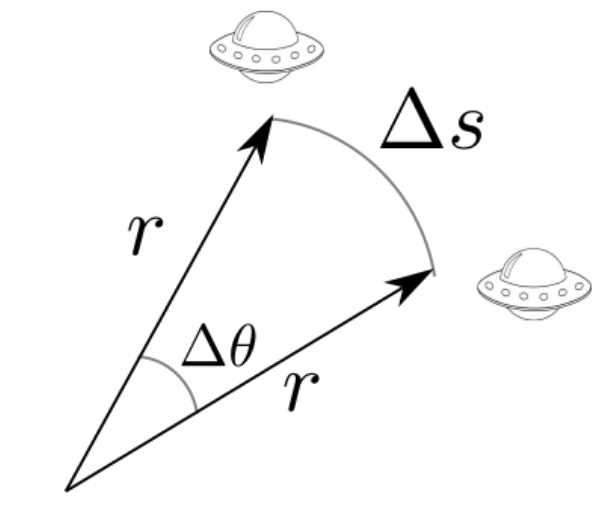
\includegraphics[scale=0.5]{media/tangential_vel.png}\\
{\small som viser en liten forflytning $\Delta s$ av romskipet i retning av enhetsvektoren $\vec{e}_\theta$. Det er altså en forflytning ortogonalt på posisjonsvektoren som skjer i løpet av et kort tidsrom $\Delta t$. Hvordan kan du bruke disse to størrelsene til å definere $v_\theta$, og hvordan kan du skrive $\Delta s$ uttrykt med $r$ og $\Delta\theta$?}\hyperlink{hastighet6}{\pagebutton{Neste side}}
\end{frame}

\renewcommand{\headline}{\small Forberede 2-legemeproblem: angulærmoment}

\begin{frame}
\label{hastighet6}
\lastpagebutton{hastighet5}
Hvis du har tenkt deg nøye om, se på \href{https://www.uio.no/studier/emner/matnat/astro/AST2000/h20/undervisningsressurser/interaktive-forelesningsnotater/1b/videoer/video1b_3.mp4}{denne videoen her} for en forklaring.\\
{\bf Bruk nå uttrykket du har funnet for $v_\theta$ til å vise at spinn (angulærmoment) per masse for romskipet, $h$, er gitt ved $h=r^2\dot\theta$.} Spinn per masse er definert som
\[
\vec{h}=\frac{\vec{r}\times\vec{p}}{m}
\]
der $\vec{p}=m\vec{v}$ er bevegelsesmengden til romskipet og $m$ er massen. Denne størrelsen skal vi bruke mye fremover. Hvis du har forstått alt vi har gått gjennom frem til nå, så bør du få til å vise at $h=r^2\dot\theta$ (bruk uttrykket vi har funnet for $\vec{v}$). Hvis ikke, så er det {\bf svært viktig} at du kontakter foreleser eller gruppelærer for hjelp før du går videre!
\hyperlink{blue_nytema5}{\pagebutton{Neste side}}
\end{frame}

\renewcommand{\headline}{\small Keplers lover}
{
\setbeamercolor{background canvas}{bg=blue}
\begin{frame}
\label{blue_nytema5}
\hyperlink{hastighet6}{\pagebutton{\small Forrige side}}
\nytemaside{red_kepler5b}
\textcolor{yellow}{Keplers lover... De kan da vel alle? Hmmm, vel, har ihvertfall hørt om dem...}\\
\vspace*{0.5cm}
\hyperlink{kepler}{\pagebutton{men hvordan var de nå igjen da...}}
\end{frame}
}

\begin{frame}
\label{kepler}
\lastpagebutton{hastighet6}
\addtocounter{pageno}{-1}
Nå begynner vi å nærme oss \textcolor{red}{den analytiske utledning av baner} her, men før i setter igang, har du hørt om Keplers lover?
\hyperlink{kepler_b}{\pagebutton{JA!}}\ \ \ \ \ \hyperlink{kepler_c}{\pagebutton{NEI!}}
\textcolor{white}{
OK, her er de:\\
PlanetenePlanetene går i ellipsebaner med sola i det ene brennpunktet\\
En linjePlanetene fra sola til planeten sveiper ut like store areler i løpet av like store tidsrom\\
PlaneteneOmløpsperioden (gitt i jordår) i annen potens  er lik store halvakse i ellipsebanen (gitt i AU) i tredje potens, $P^2=a^3$.\\
Se gjerne {denne videoen} hvis du er usikker på hva lovene sier. {\bf Hvis du allerede vet, ikke kast bort tid på videoen.}\\
Se gjerne {denne videoen} hvis du er usikker på hva lovene sier. {\bf Hvis du allerede vet, ikke kast bort tid på videoen.}\\
  Se gjerne {denne videoen} hvis du er usikker på hva lovene sier. {\bf Hvis du allerede vet, ikke kast bort tid på videoen.}\\
}
\end{frame}


\begin{frame}
\label{kepler_b}
\lastpagebutton{hastighet6}
\addtocounter{pageno}{-1}
Nå begynner vi å nærme oss \textcolor{red}{den analytiske utledning av baner} her, men før i setter igang, har du hørt om Keplers lover?
{\pagebutton{JA!}}\ \ \ \ \ {\pagebutton{NEI!}}\\
Så fint da! Da husker du kanskje også omtrent hva Keplers lover sier? Tenk deg godt om før du går videre!!!\\
\hyperlink{kepler_c}{\pagebutton{Få se Keplers lover da vel!}}
\textcolor{white}{
OK, her er de:\\
PlanetenePlanetene går i ellipsebaner med sola i det ene brennpunktet\\
En linjePlanetene fra sola til planeten sveiper ut like store areler i løpet av like store tidsrom\\
PlaneteneOmløpsperioden (gitt i jordår) i annen potens  er lik store halvakse i ellipsebanen (gitt i AU) i tredje potens, $P^2=a^3$.\\
Se gjerne {denne videoen} hvis du er usikker på hva lovene sier. {\bf Hvis du allerede vet, ikke kast bort tid på videoen.}\\
}
\end{frame}

\begin{frame}
\label{kepler_c}
\lastpagebutton{hastighet6}
\addtocounter{pageno}{-1}
Nå begynner vi å nærme oss \textcolor{red}{den analytiske utledning av baner} her, men før i setter igang, har du hørt om Keplers lover?
{\pagebutton{JA!}}\ \ \ \ \ {\pagebutton{NEI!}}\\
\vspace*{2cm}
OK, her er de:\\
\begin{enumerate}
\item Planetene går i ellipsebaner med sola i det ene brennpunktet
\item En linje fra sola til planeten sveiper ut like store areler i løpet av like store tidsrom
\item Omløpsperioden (gitt i jordår) i annen potens  er lik store halvakse i ellipsebanen (gitt i AU) i tredje potens, $P^2=a^3$.
\end{enumerate}
Se gjerne \href{https://www.uio.no/studier/emner/matnat/astro/AST2000/h20/undervisningsressurser/interaktive-forelesningsnotater/1b/videoer/video1b_4.mp4}{denne videoen} hvis du er usikker på hva lovene sier. {\bf Hvis du allerede vet, ikke kast bort tid på videoen.}
\hyperlink{kepler0b}{\pagebutton{Neste side}}
\end{frame}

\begin{frame}
\label{kepler0b}
\dlastpagebutton{kepler}
{\Large
Merket du deg forresten en viktig ting på forrige side og i videoen? I astrofysikken bruker vi enheten AU (Astronomial Unit), astronomiske enheter, veldig mye så lær deg med en gang hva denne betyr:}
\begin{block}{\bf Astronomisk enhet (AU)}
{\large Er middelavstanden mellom sola og jorda, ca. 150 millioner km!}
\end{block}
\hyperlink{kepler1}{\pagebutton{Neste side}}
\end{frame}

\renewcommand{\headline}{\small Ellipser}

\begin{frame}
\label{kepler1}
\lastpagebutton{kepler0b}
\addtocounter{pageno}{-1}
Når vi snakker om ellipsebaner, husker du forresten formelen for en ellipse...?
\hyperlink{kepler1_b}{\pagebutton{Trykk her når du har tenkt deg om...}}\\
\textcolor{white}{
Ellipser:
\[
\frac{x^2}{a^2}+\frac{y^2}{b^2}=1
\]
der $a$ er \textcolor{white}{store halvakse (semi major axis)} og $b$ er \textcolor{white}{lille halvakse (semi minor axis)}.\\
\hspace*{18cm}
{Neste side}}\\
\end{frame}

\begin{frame}
\label{kepler1_b}
\lastpagebutton{kepler0b}
\addtocounter{pageno}{-1}
Når vi snakker om ellipsebaner, husker du forresten formelen for en ellipse...?
{\pagebutton{Trykk her når du har tenkt deg om...}}\\
Ellipser:
\[
\frac{x^2}{a^2}+\frac{y^2}{b^2}=1
\]
der $a$ er \textcolor{red}{store halvakse (semi major axis)} og $b$ er \textcolor{red}{lille halvakse (semi minor axis)}.
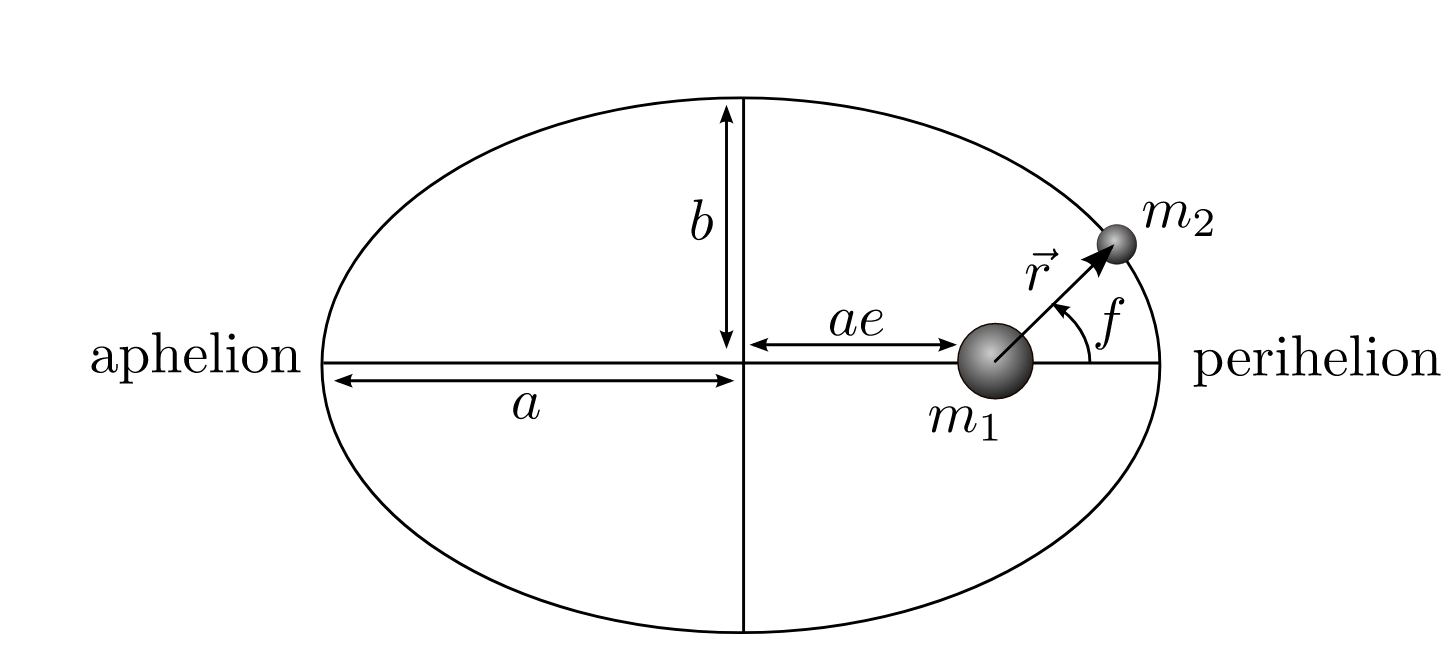
\includegraphics[scale=0.4]{media/ellipse.png}\hspace*{-2cm}\hyperlink{kepler2}{\pagebutton{Neste side}}
\end{frame}







\begin{frame}
\label{kepler2}
\dlastpagebutton{kepler1}
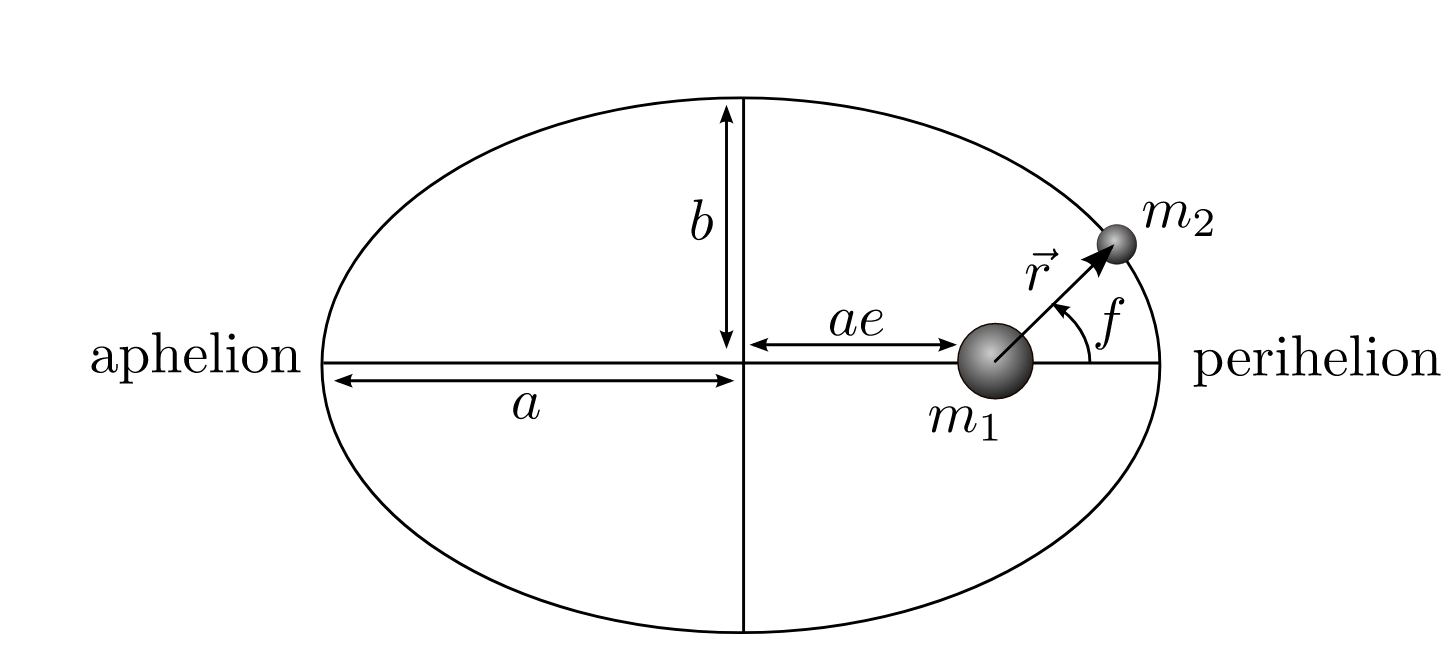
\includegraphics[scale=0.4]{media/ellipse.png}\\
I tillegg til halvaksene bør du kjenne til begrepet \textcolor{red}{brennpunkt}. Denne er markert med massen $m_1$ på figuren. En ellipse har to brennpunkter, begge ligger i en avstand $ae$ fra sentrum langs store halvakse. Størrelsen $e$ kaller vi \textcolor{red}{eksentrisiteten} og sier noe om hvor avlang ellipsen er.
\hyperlink{kepler3}{\pagebutton{Neste side}}
\end{frame}


\begin{frame}
\label{kepler3}
\lastpagebutton{kepler2}
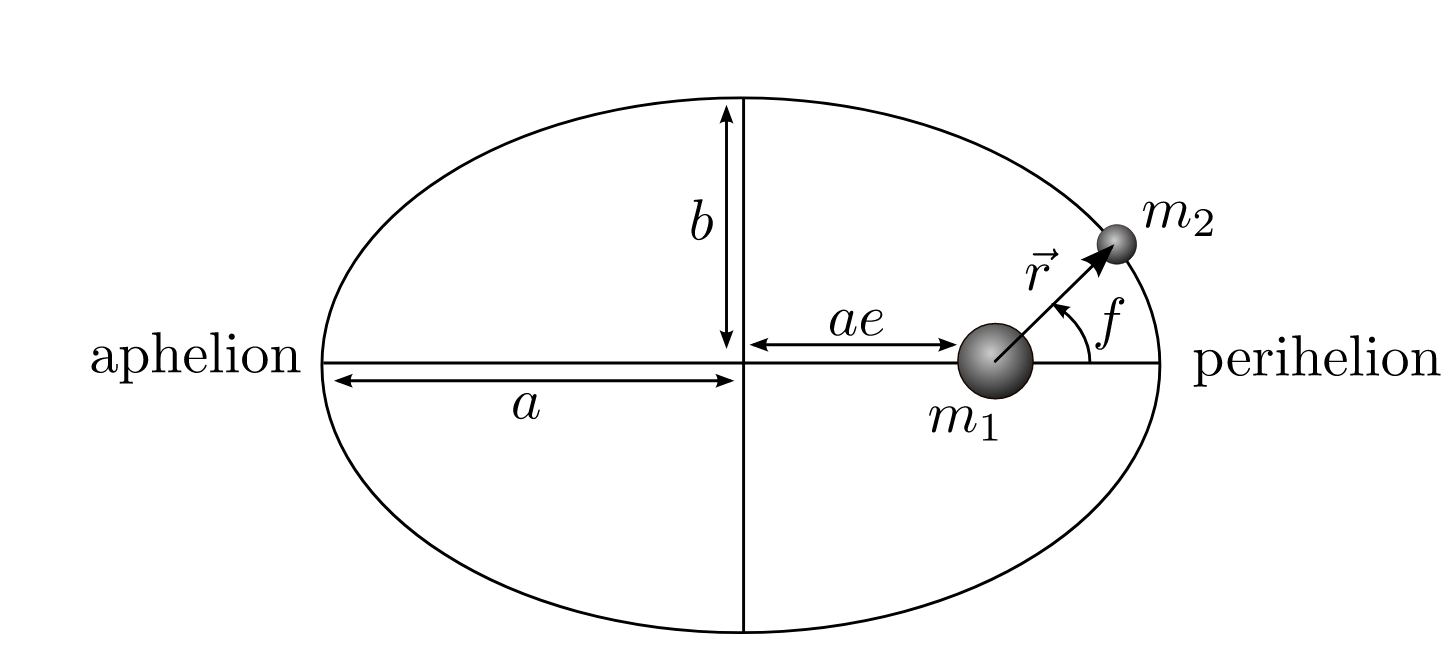
\includegraphics[scale=0.4]{media/ellipse.png}\\
{
\small
Sammenhengen mellom eksentrisiteten og lille og store halvakse er gitt ved
\[
e=\sqrt{1-\left(\frac{b}{a}\right)^2}
\]
Vi ser at hvis vi har en sirkel så må store og lille halvakse være like store, $a=b$, og da ser vi fra denne formelen at $e=0$. Hvis derimot $a$ er mye større enn $b$ så har vi en veldig avlang ellipse og da gir formelen oss at eksentrisiteten er veldig stor, $e\rightarrow1$. Eksentrisiteten er alltid $e<1$.
}
\hyperlink{kepler4}{\pagebutton{Neste side}}
\end{frame}

\begin{frame}
\label{kepler4}
\lastpagebutton{kepler3}
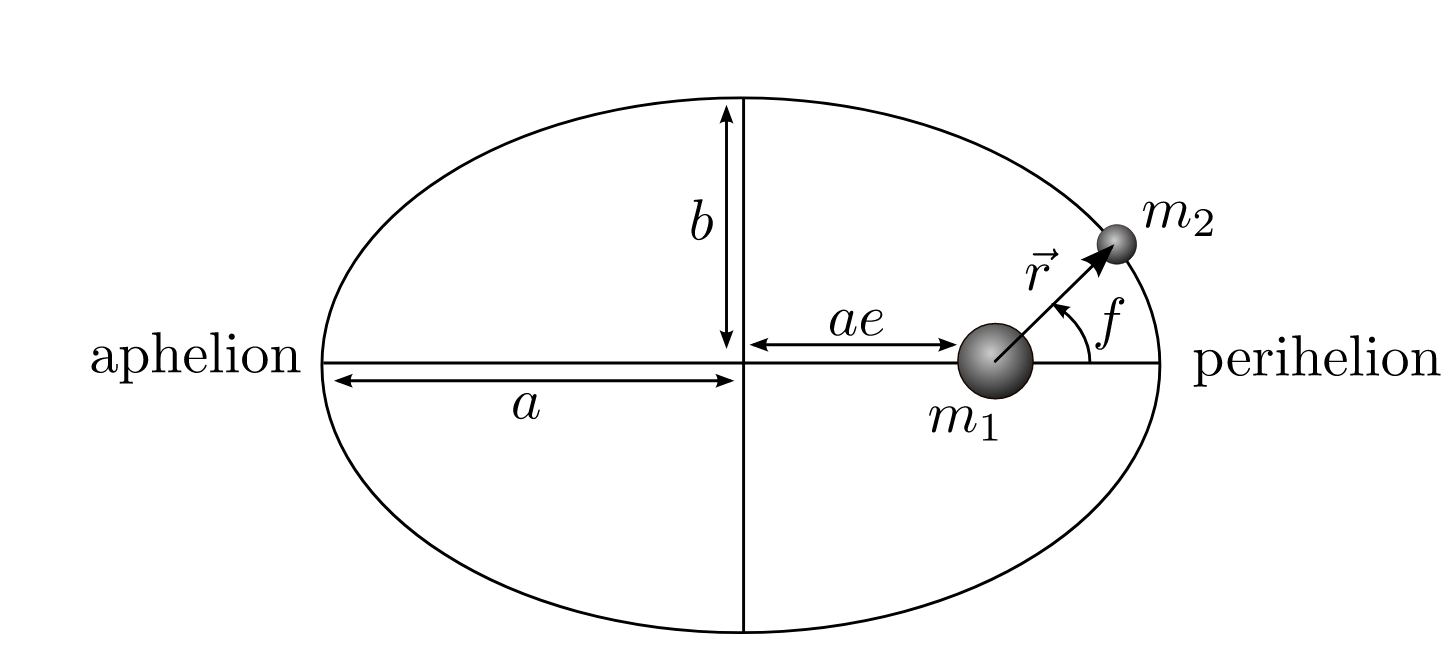
\includegraphics[scale=0.4]{media/ellipse.png}\\
Når vi snakker om ellipsebanene i Keplers første lov, enten det gjelder planetenes baner rundt sola eller en satelitts bane rundt en planet, så ligger altså den ene massen $m_1$ i brennpunktet og den andre massen $m_2$ går i ellipsebane rundt. Det er noen ord til som du må lære her: \textcolor{red}{periapsis} er punktet i ellipsebanen der objektene er nærmest hverandre og \textcolor{red}{apoapsis} er punktet i ellipsebanen der de er lengst fra hverandre. For en planets bane rund sola så brukes ordene \textcolor{red}{perihel} og \textcolor{red}{aphel} isteden.

\hyperlink{kepler4b}{\pagebutton{Neste side}}
\end{frame}

\begin{frame}
\label{kepler4b}
\lastpagebutton{kepler4}
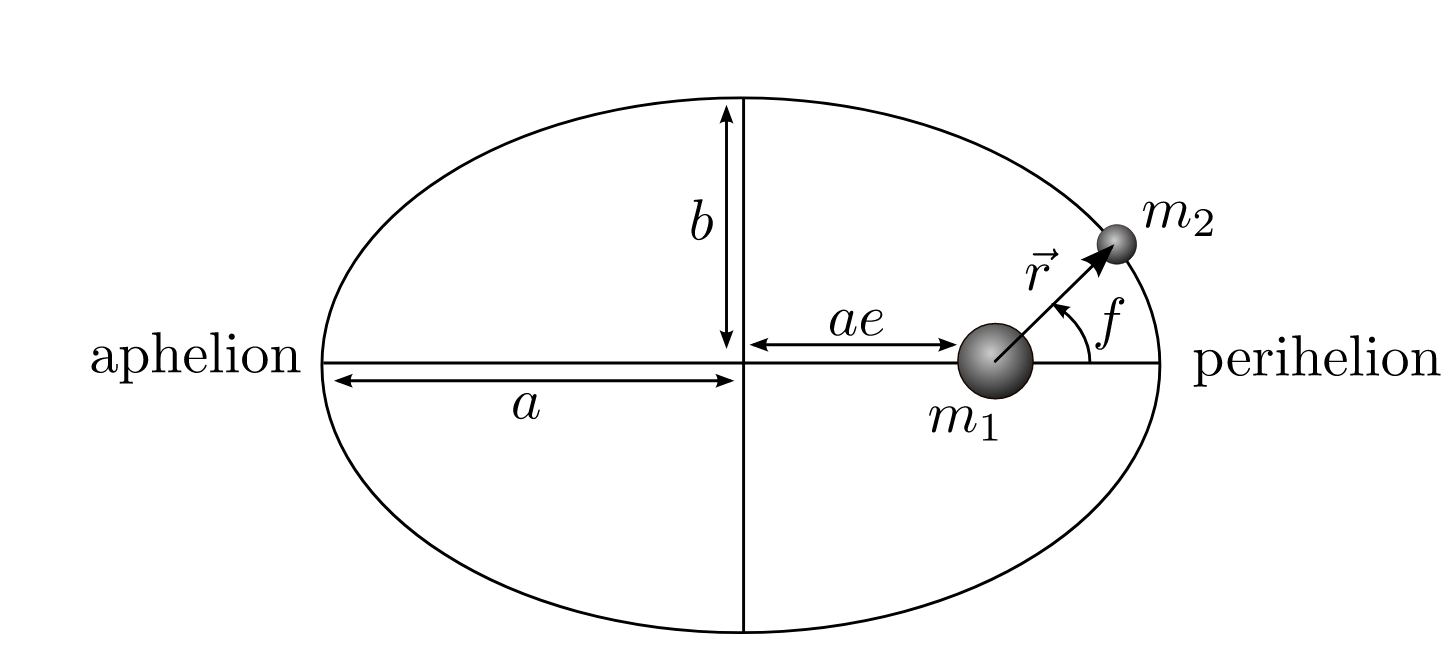
\includegraphics[scale=0.3]{media/ellipse.png}\\
{
\small
En liten ting til om ellipser. I polarkoordinater kan du skrive ellipseformelen på denne måten (hvis du er interessert i hvordan du går fra uttrykket i xy-koordinater til polarkoordinater, så ta en kikk i de vanlige forelesningsnotatene, det er ikke pensum):
\[
r(f)=\frac{a(1-e^2)}{1+e\cos{f}}
\]
der $r(f)$ er lengden av vektoren $\vec{r}$ i figuren, altså avstanden fra brennpunktet til objekt $m_2$ og vinkelen $f$ er definert som vinkelen mellom $\vec{r}$ og vektoren som går fra brennpunktet i $m_1$ til perihel. Hvis vi setter inn $f=0$ her hva får du da for lengden $r$? Stemmer det overens med det du ser geometrisk på figuren? Og hva med $f=\pi$? ({\bf hint:} avstand fra sentrum til brennpunkt er $ae$.)\\
\hyperlink{pause}{\pagebutton{Neste side}}
}
\end{frame}

{
\setbeamercolor{background canvas}{bg=cyan}
\begin{frame}
\label{pause}
\hyperlink{kepler4b}{\pagebutton{\small Forrige side}}
{\Large
\centerline{TID FOR KAFFEPAUSE!!!}
\centerline{
\includegraphics[scale=4]{media/drink-coffee.png}}\\

Ut å strekke på bena. Inn med litt koffein...\\
\vspace*{0.5cm}
Ihvertfall 10 min...
}\\
\vspace*{0.5cm}
Kommer omtrent hit (kanskje 4 slides til) på en fysisk forelesning (en dobbelttime). Gå litt videre, og så gir du deg for idag (kanskje etter den første videoen)\\
\vspace*{0.5cm}
\hyperlink{kepler5}{\pagebutton{Jeg lover, jeg har tatt pause og er klart til å fortsette}}
\end{frame}
}


\renewcommand{\headline}{\small Forberede 2-legemeproblemet}




\begin{frame}
\label{kepler5}
\lastpagebutton{kepler4b}
\addtocounter{pageno}{-1}
Da er vi klare til å begynne utledningen av Keplers første lov! Eller???\\
{
\small
En rask sjekk om du har oversikt over det som trengs
\begin{itemize}
\item Du kjenner til enhetsvektorene $\vec{e}_r$ og $\vec{e}_\theta$ og hvordan disse er definert?
\item Du forstår hvordan du deriverer disse enhetsvektorene?
\item Du forstår hvordan du kan derivere posisjonsvektoren $\vec{r}$ og dermed finne hastighetsvektoren $\vec{v}$?
\item Du forstår forskjellen mellom radiell og tangensiell hastighet og kan uttrykke disse ved hjelp av $r$ og $\theta$ samt disses derivert?
\item Du kan kan uttrykket for spinn per masse ($h$) uttrykt ved hjelp av $r$ og $\theta$ samt disses derivert? Og kan utlede dette?
\item Du vet hva lille/store halvakse, eksentrisitet, brennpunkt, apoapsis/aphel, periapsis/perihel er?
\end{itemize}
}
\hyperlink{blue_nytema6}{\pagebutton{ÅJA, dette kan jeg, la oss sette igang med utledningen!}}\\
\hyperlink{kepler5_b}{\pagebutton{Njaaaa...jeg trenger kanskje litt repetisjon}}\\
\textcolor{white}{\small Bruk 'forrige side'-knappene til å gå bakover og repetere. Dette er viktig, ikke gå videre før du har kontroll, da blir alt bare så mye vanskeligere.}
\end{frame}


\begin{frame}
\label{kepler5_b}
\lastpagebutton{kepler4b}
\addtocounter{pageno}{-1}
Da er vi klare til å begynne utledningen av Keplers første lov! Eller???\\
{
\small
En rask sjekk om du har oversikt over det som trengs
\begin{itemize}
\item Du kjenner til enhetsvektorene $\vec{e}_r$ og $\vec{e}_\theta$ og hvordan disse er definert?
\item Du forstår hvordan du deriverer disse enhetsvektorene?
\item Du forstår hvordan du kan derivere posisjonsvektoren $\vec{r}$ og dermed finne hastighetsvektoren $\vec{v}$?
\item Du forstår forskjellen mellom radiell og tangensiell hastighet og kan uttrykke disse ved hjelp av $r$ og $\theta$ samt disses derivert?
\item Du kan kan uttrykket for spinn per masse ($h$) uttrykt ved hjelp av $r$ og $\theta$ samt disses derivert? Og kan utlede dette?
\item Du vet hva lille/store halvakse, eksentrisitet, brennpunkt, apoapsis/aphel, periapsis/perihel er?
\end{itemize}
}
\hyperlink{blue_nytema6}{\pagebutton{ÅJA, dette kan jeg, la oss sette igang med utledningen!}}\\
{\pagebutton{Njaaaa...jeg trenger kanskje litt repetisjon}}\\
\textcolor{red}{\small Bruk 'forrige side'-knappene til å gå bakover og repetere. Dette er viktig, ikke gå videre før du har kontroll, da blir alt bare så mye vanskeligere.}
\end{frame}


\renewcommand{\headline}{\small Løse 2-legemeproblemet}
{
\setbeamercolor{background canvas}{bg=blue}
\begin{frame}
\label{blue_nytema6}
\hyperlink{kepler5}{\pagebutton{\small Forrige side}}
\nytemaside{0}
\textcolor{yellow}{Keplers lover... De kan da vel alle? Hmmm, vel, har ihvertfall hørt om dem...}\\
\vspace*{0.5cm}
\hyperlink{red_kepler5b}{\pagebutton{men hvordan var det nå igjen da...}}
\end{frame}
}


{
\setbeamercolor{background canvas}{bg=red}
\begin{frame}
\label{red_kepler5b}
\dlastpagebutton{kepler5}
Vi skal i det følgende løse det som vi kaller {\bf 2-legeme-problemet}:\\
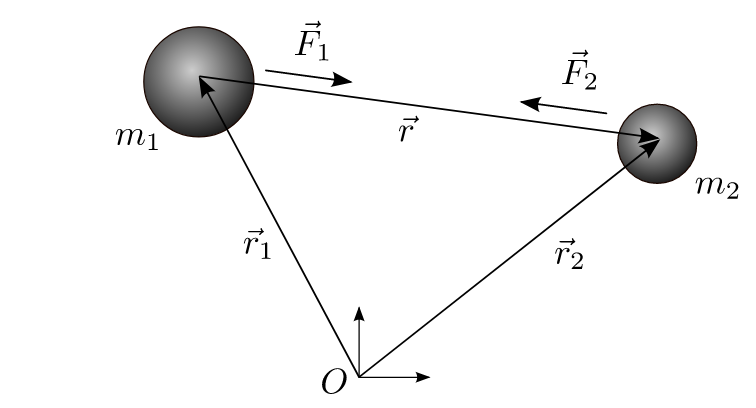
\includegraphics[scale=0.4]{media/forces.png}\\
{\bf To legemer med masse $m_1$ og $m_2$ påvirker hverandre kun med gravitasjonskrefter. Det virker ingen eksterne krefter. Initialposisjonene og initialhastighetene til begge legemene er kjent.} For å gjøre utledningen enklere skal vi først sette oss på $m_1$ og utlede bevegelsen til $m_2$ sett ifra $m_1$. Dermed trenger vi kun å se på bevegelsen til {\it et} legeme. Etter det skal vi se på bevegelsene til begge legemene.\\
På figuren ser du at vektoren $\vec{r}$ peker fra $m_1$ til $m_2$. {\bf Når vi setter oss på $m_1$ og definerer origo der, så er denne $\vec{r}$ altså poisjonsvektoren til $m_2$. Når vi har funnet hvordan $\vec{r}(t)$ endrer seg som funksjon av tiden så har vi løst 2-legeme-problemet sett fra objekt $m_1$.}
\hyperlink{kepler6}{\pagebutton{Neste side}}
\end{frame}
}


\begin{frame}
\label{kepler6}
\lastpagebutton{red_kepler5b}
I \href{https://www.uio.no/studier/emner/matnat/astro/AST2000/h20/undervisningsressurser/interaktive-forelesningsnotater/1b/videoer/video1b_5.mp4}{denne videoen} begynner vi utledningen av løsningen på 2-legemeproblemt. Vi diskuterer krefter på objektene og bruker Newtons lover inkludert gravitasjonsloven til å komme frem til
\[
\ddot{\vec{r}}+m\frac{\vec{r}}{r^3}=0
\]
der vi har definert $m=G(m_1+m_2)$ og $r=|\vec{r}|$ der $\vec{r}$ peker fra masse $m_1$ til masse $m_2$.\\
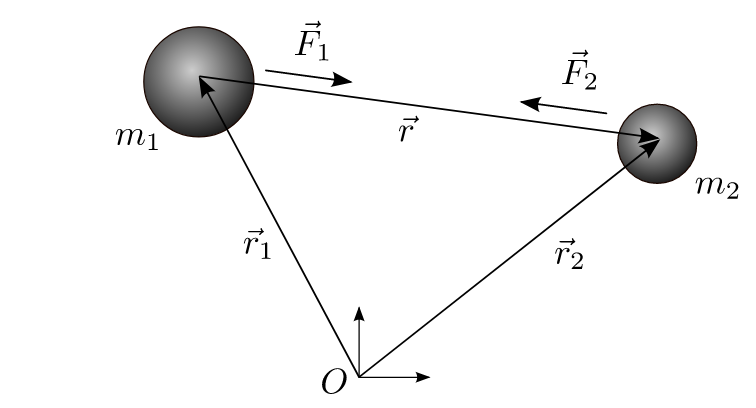
\includegraphics[scale=0.4]{media/forces.png}\\
Dette {\bf bevegelseslikningen} for systemet vårt. Det er en differensiallikning i funksjonen $\vec{r}(t)$. Hvis vi klarer å løse for $\vec{r}(t)$, har vi funnet bevegelsen til $m_2$ i forhold til $m_1$ og dermed løst 2-legemeproblemet sett ifra $m_1$.
\hyperlink{kepler7}{\pagebutton{Neste side}}
\end{frame}

\begin{frame}
\label{kepler7}
\lastpagebutton{kepler6}
{\small For å kunne løse denne likningen, så trenger vi å innføre enhetsvektorer. Det viser seg at det er lettere å jobbe med $\vec{e}_r$ og $\vec{e}_\theta$ her! Ta en titt på denne figuren:}\\
\begin{columns}
\column{0.5\textwidth}
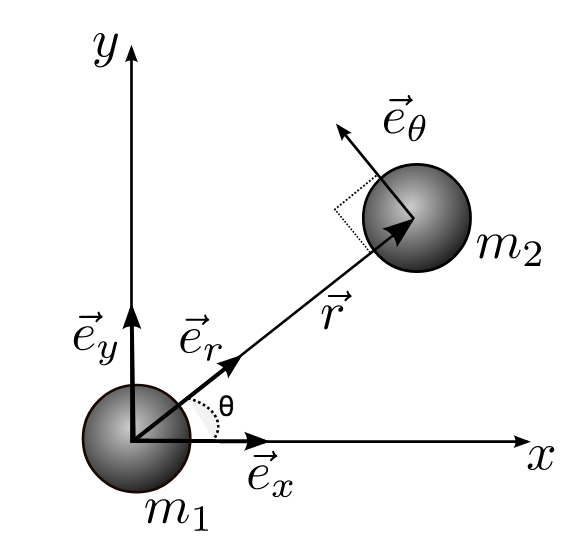
\includegraphics[scale=0.37]{media/unityvectors_on_m1m2.png}
\column{0.5\textwidth}
{\Large 
\[
\hspace*{-4cm}\ddot{\vec{r}}+m\frac{\vec{r}}{r^3}=0
\]
}
\end{columns}
{\small Vi har nå definert origo i sentrum av $m_1$ slik at $\vec{r}$ er en posisjonsvektor som peker på $m_2$. Sett inn enhetsvektorer, deriver og dobbeltderiver $\vec{r}$ og se om du klarer å komme frem til: {\bf (hint: gå baklengs fra dette svaret for å sammenlikne!)}
\[
(\ddot{r}-r\dot{\theta}^2)\vec{e}_r+\frac{1}{r}\frac{d}{dt}(r^2\dot{\theta})\vec{e}_\theta=-\frac{m}{r^2}\vec{e}_r.
\]
Flere hint: start fra uttryket for $\dot{\vec{r}}$ og husk at $\dot{\vec{e}}_r = \dot\theta\vec{e}_\theta$ og $\dot{\vec{e}}_\theta = -\dot\theta\vec{e}_r$. Hvis du ikke får det til, ta en titt på \href{https://www.uio.no/studier/emner/matnat/astro/AST2000/h20/undervisningsressurser/interaktive-forelesningsnotater/1b/videoer/video1b_6.mp4}{denne videoen her} , men \textcolor{red}{\bf kun når du har gjort et skikkelig forsøk selv!}.}
\hyperlink{kepler8}{\pagebutton{Neste side}} ({\bf Feil i videoen: det står $r^3$ under brøkstreken på høyre side, det skal være $r^2$ som i likningen rett over)}
\end{frame}

\begin{frame}
\label{kepler8}
\lastpagebutton{kepler7}
\[
(\ddot{r}-r\dot{\theta}^2)\vec{e}_r+\frac{1}{r}\frac{d}{dt}(r^2\dot{\theta})\vec{e}_\theta=-\frac{m}{r^2}\vec{e}_r.
\]
Se nøye på denne likningen! Se om du kan bruke den til å trekke følgende konklusjoner:
\begin{block}{Vi har gjort om vektorlikningen til to skalare likninger som sier:}
\begin{itemize}
\item Vi har utledet at spinn per masse ($h$) er en bevart størrelse.
\item Vi har kommet til at
\[
\ddot{r}-r\dot{\theta}^2=-\frac{m}{r^2}
\]
\end{itemize}
\end{block}
Hvis du ikke ser hvordan vi kommer frem til dette, så \href{https://www.uio.no/studier/emner/matnat/astro/AST2000/h20/undervisningsressurser/interaktive-forelesningsnotater/1b/videoer/video1b_7.mp4}{kikk på denne videoen}.
\hyperlink{kepler9}{\pagebutton{Neste side}}
\end{frame}

\begin{frame}
\label{kepler9}
\lastpagebutton{kepler8}
Nå nærmer vi oss slutten her!\\
Vi skal nå gjøre to steg:
\begin{enumerate}
\item vi skal bruke $\theta$ som variabel isteden for tiden $t$. Hvis vi kun er interessert i formen på banen og ikke hvor objektet er til en gitt tid, så holder det å få ut svaret $r(\theta)$, dvs. hva er lengden av $\vec{r}$ når vinkelen som vektoren danner med x-aksen er $\theta$? Vi skal altså ha deriverte i forhold til $\theta$ isteden for tiden.
\item For å gjøre det enklere å løse likningen, så viser det seg at det er bedre å definere $u(\theta)=\frac{1}{r(\theta)}$ og substituerer $u$ overalt der det er $r$. Vi løser for $u(\theta)$ og til slutt setter vi inn for $r$ igjen.
\end{enumerate}
Du skal nå få prøve deg litt selv, før du får svaret...
\hyperlink{kepler10}{\pagebutton{Neste side}}
\end{frame}

\begin{frame}
\label{kepler10}
\lastpagebutton{kepler9}
{\bf Den delen av utledningen som står på denne siden er ikke superviktig, du kommer ikke til å bli spurt om dette i oppgavene eller på eksamen. Men det er kult å ha sett det en gang. Gå gjerne fort gjennom hvis du ikke er interessert.}
Deriver $u$ med hensyn på $\theta$, bruk kjerneregel til å forbinde denne med $\dot r$ og se om du klarer å få:
\[
\frac{du(\theta)}{d\theta}=-\frac{\dot r}{h}
\]
der $h$ er spinn per masse. Og deriverer du en gang til skal du få:
\[
\frac{d^2u(\theta)}{d\theta^2}=-\frac{\ddot r}{h\dot\theta}
\]
Hvis du nå setter inn $\ddot r$ fra likningen vi fant over ($\ddot{r}-r\dot{\theta}^2=-\frac{m}{r^2}$), klarer du å få
\[
\frac{d^2u(\theta)}{d\theta^2}+u=\frac{m}{h^2}
\] 
Var disse stegene litt vanskelige? Det var meningen! Ikke bruk mye tid på dette, her er det mer matematisk triksing enn det er fysikk. \href{https://www.uio.no/studier/emner/matnat/astro/AST2000/h20/undervisningsressurser/interaktive-forelesningsnotater/1b/videoer/video1b_8.mp4}{HER} finner du en video som forklarer det.
\hyperlink{kepler11}{\pagebutton{Neste side}}
\end{frame}

\begin{frame}
\label{kepler11}
\begin{columns}
\column{0.5\textwidth}
\lastpagebuttonx{kepler10}
\headlinebutton{\headline}\\
Før vi går videre, la oss snakke om noe helt annet. Har du hørt om {\it harmonisk oscillator?}. Se på denne situasjonen:\\
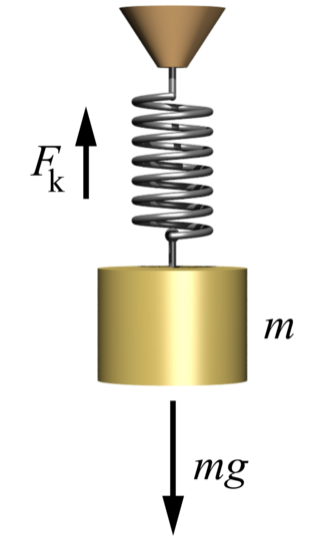
\includegraphics[scale=0.4]{media/harmosc.png}
Hvis vi antar at vi har en x-akse som går nedover her, er du enig i at følgende likning beskriver x-posisjonen til loddet:
\[
F=ma=m\ddot x=-kx+mg
\]
\column{0.5\textwidth}
der $m$ er massen til loddet, $kx$ er fjærkraften som virker oppover, $k$ er fjærkonstanten, jo større $x$ er jo større er kraften, og $mg$ er vanlig tyngdekraft (vi antar $g$ konstant her). Hvis vi deler med $m$ her og flytter over får vi:

\[
\frac{d^2x}{dt^2}+\frac{k}{m}x=g
\]
som er likningen for en harmonisk oscillator. Hvis vi setter $k/m=1$ så ser vi at vi har nøyaktig samme type differensiallikning:
\[
\frac{d^2u(\theta)}{d\theta^2}+u=\frac{m}{h^2}
\]
Dette er også en harmonisk oscillator.
\hyperlink{kepler12}{\pagebutton{Neste side}}
\end{columns}
\end{frame}


\begin{frame}
\label{kepler12}
\lastpagebutton{kepler11}
Vi forstår at løsningen er oscillerende: loddet kommer til å svinge opp og ned ettersom tyngden drar det nedover og fjæren oppover så få vi en svingene bevegelse. Det samme må altså skje med $u(\theta$), ettersom $\theta$ endrer seg så må $u$ (og dermed $r$) bli større og mindre. Dette stemmer jo med en ellipse: planeten går fra perihel til aphel og dermed svinger $r$ (avstanden til brenpunktet) mellom minste og største verdi, akkurat som loddet. Men kan du se en analytisk løsning av denne likningen?\\
Hvis du først setter konstanten lik 0 og flytter over på høyre side så står det:
\[
\frac{d^2u(\theta)}{d\theta^2}=-u
\]
Ser du en løsning av denne likningen? Her har vi jo en funksjon $u$ som er slik at hvis du deriverer den to ganger så får vi $-u$ tilbake, hva må det være?\\
\hyperlink{kepler13}{\pagebutton{Tenk deg godt om! Ikke trykk her før du har svaret!}}
\end{frame}

\begin{frame}
\label{kepler13}
\lastpagebutton{kepler12}
Ganske riktig ja! En cosinus eller sinus er jo akkurat slik at hvis du deriverer den to ganger så få du tilbake minus funksjonen selv. Hva hvis vi nå tar med konstantleddet da. Hva blir løsningen av denne likningen?
\begin{block}{\bf Likningen for harmonisk oscillator for tolegemeproblemet}
\[
\frac{d^2u(\theta)}{d\theta^2}+u=\frac{m}{h^2}
\]
\end{block}
Prøv deg litt frem på papir, maks 2-3 minutter, se hvor langt du kommer...
\hyperlink{red_kepler14}{\pagebutton{Nå har jeg prøvd meg litt!}}
\end{frame}


{
\setbeamercolor{background canvas}{bg=red}
\begin{frame}
\label{red_kepler14}
\lastpagebutton{kepler13}
Hvis du har funnet en løsning, er du {\bf helt} sikker på at du har funnet riktig løsning?. Før du går videre nå, ta din løsning $u(\theta)$ og dobbeltderiver den!
Er svaret du får lik:
\[
\frac{m}{h^2}-u
\]
???\\
Helt sikker?
\hyperlink{kepler15}{\pagebutton{Neste side}}
\end{frame}
}

\begin{frame}
\label{kepler15}
\lastpagebutton{red_kepler14}
\addtocounter{pageno}{-1}
Da skulle du ha fått følgende svar:
\[
u(\theta)=\frac{m}{h^2}+A\cos{(\theta-\omega)}
\]
hvor $A$ og $\omega$ er integrasjonskonstanter. Ble det riktig?\\
Hvis vi nå omdøper integrasjonskontantene og gjør om til $r(\theta)$ ved $r=1/u$ så få vi da:
\[
r(f)=\frac{p}{1-e\cos{f}}
\]
hvor vi har definert $f=\theta-\omega$, $p=h^2/m$ og $e=Ap$. MERK at $p$ her ikke har noe med bevegelesmengde å gjøre!
Ser du noe kjent med dette uttrykket? Kan du skrive det litt om for å få noe kjent?\\
\textcolor{red}{(MERK deg også definisjonen $p=h^2/m$ her, den kommer du til å bruke i neste forelesning!)}\\
\hyperlink{kepler15_2}{\pagebutton{Neste side}}
\end{frame}

\begin{frame}
\label{kepler15_2}
\lastpagebutton{kepler15}
\textcolor{red}{{\bf HØØØØ!!DU!! Nå duppet du av litt, vi tar denne sliden EN gang til:} her var det mange konstanter og greier, og lett å gå surr. Du trenger ikke huske alle disse konstantene, men du bør forstå hva som foregår her. {\bf Så les gjennom EN gang til og smak litt på ordene...}}\\
Da skulle du ha fått følgende svar:
\[
u(\theta)=\frac{m}{h^2}+A\cos{(\theta-\omega)}
\]
hvor $A$ og $\omega$ er integrasjonskonstanter. Ble det riktig?\\
Hvis vi nå omdøper integrasjonskontantene og gjør om til $r(\theta)$ ved $r=1/u$ så få vi da:
\[
r(f)=\frac{p}{1-e\cos{f}}
\]
hvor vi har definert $f=\theta-\omega$, $p=h^2/m$ og $e=Ap$. MERK at $p$ her ikke har noe med bevegelesmengde å gjøre!
Ser du noe kjent med dette uttrykket? Kan du skrive det litt om for å få noe kjent?\\
\textcolor{red}{(MERK deg også definisjonen $p=h^2/m$ her, den kommer du til å bruke i neste forelesning!)}\\
\hyperlink{kepler16}{\pagebutton{Neste side}}
\end{frame}


\begin{frame}
\label{kepler16}
\lastpagebutton{kepler15_2}
Ganske riktig ja! Hvis vi definerer en størrelse $a$ slik at $p=a(1-e^2)$ så har vi jammen
\begin{block}{\bf Keplers første lov utledet fra Newtons lover}
Planetene går i ellipsebaner
\[
r(f)=\frac{a(1-e^2)}{1-e\cos{f}}
\]
Der solen er i det ene brennpunktet
\end{block}
Dette er jo en generell løsning av 2-legemeproblemet og gjelder da for enhver banebevegelse. MEN, for ellipser så må $e=[0,1)$ men $e$ kan aldri bli 1. I denne løsningen så kan $e$ være en hvilken som helst positiv størrelse og enda være en løsning av likningen vår. Men hvis $e\ge1$ så har vi ikke en ellipse lenger! \textcolor{red}{Betyr det at det finnes løsninger av tolegemeproblemet som {\bf ikke} er ellipsebaner men andre typer baner? Som Kepler ikke visste noe om??}\\
{\Large \bf Fortsettelse følger...}
\hyperlink{feil_kepler17}{\pagebutton{Neste side}}
\end{frame}

{
\setbeamercolor{background canvas}{bg=black}
\begin{frame}
\label{feil_kepler17}
\hyperlink{kepler16}{\pagebutton{\small Forrige side}}\href{https://nettskjema.no/a/158672}{\Changey[1][yellow]{2} \Changey[1][yellow]{-2}}
{\Huge
\textcolor{orange}{... i den neste og meget spennende forelesningen i emnet}\\
\textcolor{orange}{AST2000...}\\
\textcolor{orange}{Følg med!}\\
}
\hyperlink{oppsummering}{\pagebutton{Neste side}}
\end{frame}
}

\begin{frame}
\label{oppsummering}
\hyperlink{feil_kepler17}{\pagebutton{\small Forrige side}}\href{https://nettskjema.no/a/158672}{\Changey[1][yellow]{2} \Changey[1][yellow]{-2}}
Da er vi ved veis enda av den første forelesningen i del 1B. I den fysiske forelesningen er jeg kanskje litt over halvveis i den andre dobbelttimen på dette punktet. Du bør nå ha god oversikt over dette:
\begin{itemize}
\item posisjonsvektorer, hastighetsvektorer, enhetsvektorer i polarkoordinater
\item hvordan derivere vektorer i polarkoordinater
\item størrelser og egenskaper til en ellipse
\item vite hva en harmonisk oscillator er
\item kjenne hovedtrekkene i hvordan man løser 2-legemeproblemet
\end{itemize}
\textcolor{red}{Trykk nå gjerne på smilefjesene og si meninga di om dette interaktive forelesningsnotatet. Spesielt er jeg interessert i å vite hvor lang tid du brukte og da hva du brukte mest tid på! All ris og ros mottaes med takk for å vite om alt arbeidet med å lage disse interaktive slidene er verd det, om jeg bør fortsette med det og om det er noe jeg bør endre.}
\end{frame}


\end{document}
